%%%%%%%%%%%%%%%%%%%%%%%%%%%%%%%%%%%%%%%%%
% Stylish Article
% LaTeX Template
% Version 2.1 (1/10/15)
%
% This template has been downloaded from:
% http://www.LaTeXTemplates.com
%
% Original author:
% Mathias Legrand (legrand.mathias@gmail.com) 
% With extensive modifications by:
% Vel (vel@latextemplates.com)
%
% License:
% CC BY-NC-SA 3.0 (http://creativecommons.org/licenses/by-nc-sa/3.0/)
%
%%%%%%%%%%%%%%%%%%%%%%%%%%%%%%%%%%%%%%%%%

%----------------------------------------------------------------------------------------
%	PACKAGES AND OTHER DOCUMENT CONFIGURATIONS
%----------------------------------------------------------------------------------------

\documentclass[fleqn,12pt]{SelfArx} % Document font size and equations flushed left

\usepackage[english]{babel} % Specify a different language here - english by default

\usepackage{lipsum} % Required to insert dummy text. To be removed otherwise

%----------------------------------------------------------------------------------------
%	COLUMNS
%----------------------------------------------------------------------------------------

\setlength{\columnsep}{0.55cm} % Distance between the two columns of text
\setlength{\fboxrule}{0.75pt} % Width of the border around the abstract

%----------------------------------------------------------------------------------------
%	COLORS
%----------------------------------------------------------------------------------------

\definecolor{color1}{RGB}{0,0,90} % Color of the article title and sections
\definecolor{color2}{RGB}{0,20,20} % Color of the boxes behind the abstract and headings

%----------------------------------------------------------------------------------------
%	HYPERLINKS
%----------------------------------------------------------------------------------------

\usepackage{hyperref} % Required for hyperlinks
\hypersetup{hidelinks,colorlinks,breaklinks=true,urlcolor=color2,citecolor=color1,linkcolor=color1,bookmarksopen=false,pdftitle={Title},pdfauthor={Author}}

%----------------------------------------------------------------------------------------
%	ARTICLE INFORMATION
%----------------------------------------------------------------------------------------

\JournalInfo{6.864/6.867 Final Paper} % Journal information
\Archive{} % Additional notes (e.g. copyright, DOI, review/research article)

\PaperTitle{How Does Content Drive Viewership?} % Article title

\Authors{Dave Holtz\textsuperscript{1}, Jeremy Yang\textsuperscript{2}, Michael Zhao\textsuperscript{3*}} % Authors
\affiliation{\textsuperscript{1}\textit{dholtz@mit.edu}}
\affiliation{\textsuperscript{2}\textit{zheny@mit.edu}} 
\affiliation{\textsuperscript{3}\textit{mfzhao@mit.edu}}
\affiliation{\textsuperscript{*}\textit{Michael is also using this project to fulfill Final Project requirements for both 6.864 as well as 6.867. Dave and Jeremy are only using this project for 6.867.}}

\Keywords{} % Keywords - if you don't want any simply remove all the text between the curly brackets
\newcommand{\keywordname}{Keywords} % Defines the keywords heading name

%----------------------------------------------------------------------------------------
%	ABSTRACT
%----------------------------------------------------------------------------------------

\Abstract{Why do some webpages receive massive numbers of page views? To determine how content drives viewership, we construct a unique dataset of all articles published by the New York Times (NYT) in August 2013. Our dataset is built from 2 major components, the NYT's internal web traffic data and article content data parsed from the NYT website. We use the internal web traffic data to accurately track the number of page views of each article as well as construct a set of robust control variables such as the desk and section of each article. To build content features, we use various machine learning and statistical natural language processing techniques on our parsed article content data and construct features such as article perplexity, sentiment, reading difficulty, and indicators that denote the presence of pictures, videos, etc. Additionally, we have access to the NYT's internal website traffic data. We feed all of our constructed features to into a predictive regression model. We find that our textual features modestly improve our predictive power. However, there are still many textual features we've not yet explored due to time constraints. We believe that adding these additional features may offer more significant improvements in performance.}

%----------------------------------------------------------------------------------------

\begin{document}

\flushbottom % Makes all text pages the same height

\maketitle % Print the title and abstract box

\tableofcontents % Print the contents section

\thispagestyle{empty} % Removes page numbering from the first page

%----------------------------------------------------------------------------------------
%	ARTICLE CONTENTS
%----------------------------------------------------------------------------------------

\section{Introduction} % The \section*{} command stops section numbering

In today's digital economy, many companies are very interested in attracting users to visit their websites in order to earn ad revenue. While many factors might motivate a user to visit a particular page, certainly one important factor is the content in that webpage. This paper explores the relationship between the content of a webpage and the number of page views it ultimately ends up receiving by constructing a unique dataset of all articles published by the New York Times (NYT) during August 2013. This dataset is built from two major components: the NYT's internal web traffic data and parsed NYT article content data.

Typically, a study such as ours tends to be very difficult to conduct as either accurate measures of viewership are unavailable\footnote{While oftentimes precise viewership data tends to be not available openly, oftentimes researchers use related observables, such as Facebook likes} or the feature extraction of the content is too challenging (for example Youtube), or or both. Fortunately, our access to the the NYT's internal web traffic data allows us to exactly measure the number of page views an article receives. The web traffic data is rather rich and also includes internal meta-data that we use to build various control features. Moreover, since we are working with mostly textual data, we are able to take advantage of recent advancements in machine learning and statistical NLP to do feature extraction on article text. 

A similar study by Berger and Milkman (2012) \cite{berger2012makes} examines the relationship between content and word-of-mouth virality. They find that the emotional content of a NYT article is predictive of its virality. Using simple measures of an article's sentiment and emotionality, Berger and Milkman show that positive articles are more likely to show up on the New York Times "Most-Emailed" list. They also show that articles that evoke high physiological positive or negative arousal (such as awe or anger) tend to be more viral than articles that evoke deactivating emotions (sadness). We build on this study in two ways: first, we relate an article's content back to the number of page views it receives rather than its virality\footnote{Which companies arguably care more about since word-of-mouth virality is usually a means to increase page views}. Second, we employ more sophisticated machine learning feature extraction techniques to see if they work any better over their simple measures.
%------------------------------------------------

\section{Data}
\subsection{NYT Internal Web Traffic Data}
Our NYT internal web traffic dataset is a record of all individual user activity on the NYT website covering the period of April 3rd, 2013 to October 31st, 2013. This activity data is stored as individual lines of json and includes who (if available) accessed what page at what time. Overall, it is over 20 terabytes in size and contains over 3 billion page views. It's important to note that not all page views are content views, for example, some events that are also tracked are searches, or user account settings. Since the scope of this dataset is so large, we initially restrict this project to a single month, August 2013, with plans of including the entire dataset for future work. 

We further constrain our dataset to only include articles or blogposts published during the month of August since these are the pieces of content that have machine parsable text data. For the sake of brevity, we use articles to refer to both articles and blogposts unless we explicitly state otherwise. We make a basic first pass through the data to simply to obtain a list of urls. After cleaning up the url data to make sure we had each url mapped to a unique piece of content, we were left with a total of 6682 urls. We then parse our dataset and aggregate the number of counts each url receives. In order to make the comparison between articles fairer since an article that's been out longer will have more page views on average, we only count the number of page views received up to 7 days after publication. Given that page views tend to sharply drop off soon after publication since recency is quite important to the News, the number of page views obtained during the 7 days after an article is published represents the vast majority (usually well over 90\%) of total page views an article receives. In total, our data consists of 248,161,455 page views. As seen in Figure 1 below, the distribution of page views is highly skewed with very heavy tails. After applying a log transformation (as seen in Figure 2), our distribution looks considerably more normal. 

\begin{figure}[ht]\centering
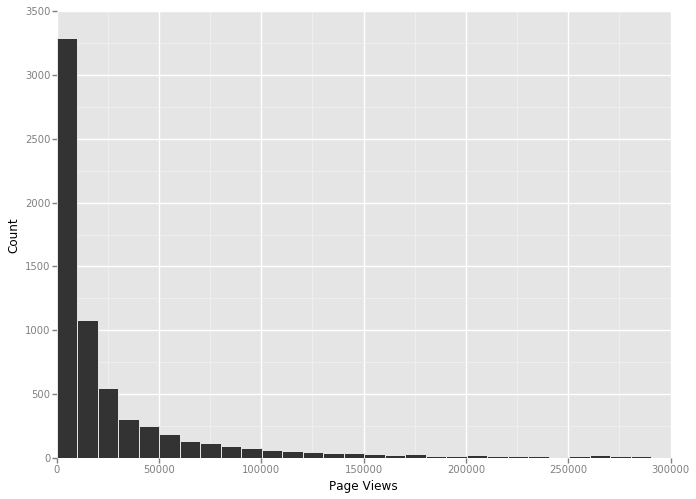
\includegraphics[width=\linewidth]{pageviews_hist}
\caption{Histogram of Articles by Number of Page Views}
\label{fig:pv_hist}
\end{figure}
% TWEAK TABLE LOOK
\begin{table}[hbt]
\caption{Page Views Distribution Summary Statistics}
\centering
\begin{tabular}{rr}
\toprule
Min               &  1\\
Max               &  2545288\\  
Mean              &  37138.8\\
Median            &  10298.5\\
StDev.         &  88972.9\\
Skew          &  9.52191\\
Kurt.          &  173.061\\
\midrule
Obs &  6682\\
\bottomrule
\end{tabular}
\end{table}

\begin{figure}[ht]\centering
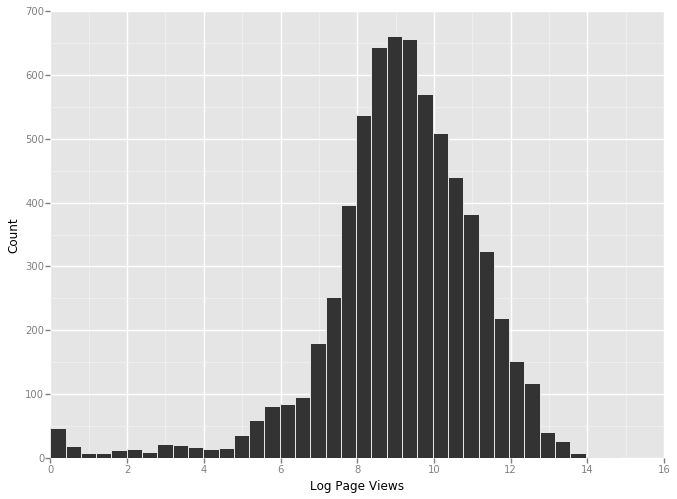
\includegraphics[width=\linewidth]{log_pageviews_hist}
\caption{Histogram of Articles by Log of Page Views}
\label{fig:lpv_hist}
\end{figure}

\begin{table}[hbt]
\caption{Log Page Views Distribution Summary Statistics}
\centering
\begin{tabular}{rr}
\toprule
Min               &  0\\
Max               &  14.74975\\  
Mean              &  9.122868\\
Median            &  9.239754\\
StDev.            &  2.028668\\
Skew              &  -1.270368\\
Kurt.             &  3.800911\\
\midrule
Obs &  6682\\
\bottomrule
\end{tabular}
\end{table}


In addition to aggregating the counts, when parser the internal web traffic data, we made sure to store various relevant article meta-data features such as the headline, time of publishing, authors, section, desk, and the NYT's internal article content description tags (if available\footnote{by this we mean that the NYT only produces these content tags only for some articles, its not a question of whether the data is available to us}).

\subsection{Parsed NYT Article Content Data}
Unfortunately, the NYT internal web traffic data does not the actual content displayed on each webpage, which is a very important aspect of our project. To resolve this issue, we used the python library ``newspaper". This library helped to scrape the html from the NYT website and extract all the raw textual data from the html. We further used some regular expressions to clean up what the library missed. In total, our 6682 articles contain 4,685,021 words of text.  We find that the distribution of article length, much like the distribution of page views, is highly skewed. We again apply a log transformation. Histograms and various summary statistics of for the distribution of article length and log article length are provided below:

\begin{figure}[ht]\centering
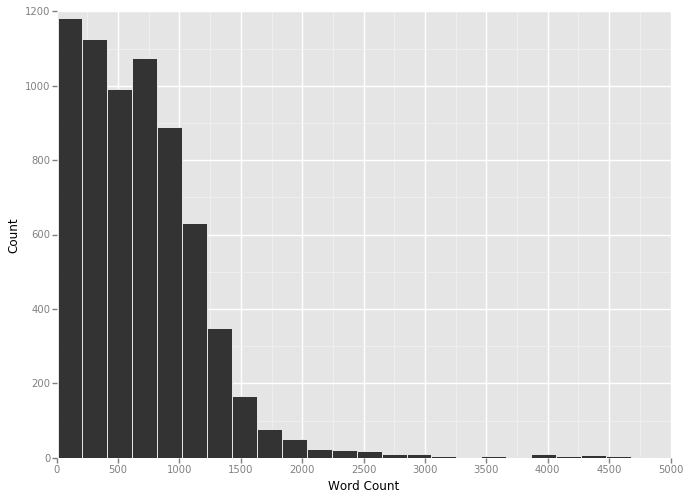
\includegraphics[width=\linewidth]{wordcount_hist}
\caption{Histogram of Articles by Word Count}
\label{fig:pv_hist}
\end{figure}

\begin{table}[hbt]
\caption{Log Page Views Distribution Summary Statistics}
\centering
\begin{tabular}{rr}
\toprule
Min               &  7\\
Max               &  8941\\  
Mean              &  701.1405\\
Median            &  625\\
StDev.            &  591.9535\\
Skew              &  3.335127\\
Kurt.             &  24.35949\\
\midrule
Obs &  6682\\
\bottomrule
\end{tabular}
\end{table}

\begin{figure}[ht]\centering
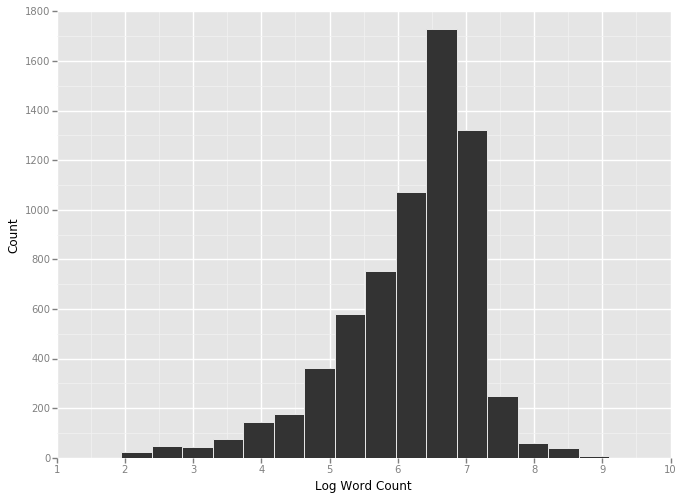
\includegraphics[width=\linewidth]{log_wordcount_hist}
\caption{Histogram of Articles by Log Word Count}
\label{fig:lpv_hist}
\end{figure}

\begin{table}[hbt]
\caption{Log Page Views Distribution Summary Statistics}
\centering
\begin{tabular}{rr}
\toprule
Min               &  1.945910\\
Max               &  9.098403\\  
Mean              &  6.181044\\
Median            &  6.437751\\
StDev.            &  1.004414\\
Skew              &  -1.178993\\
Kurt.             &  1.944611\\
\midrule
Obs &  6682\\
\bottomrule
\end{tabular}
\end{table}

In addition to extracting the raw text data, we made sure to check if the articles contained non-textual content such as pictures or videos. We created indicator variables that denote the presence of such content within an article.

%\begin{figure*}[ht]\centering % Using \begin{figure*} makes the figure take up the entire width of the page
%\includegraphics[width=\linewidth]{view}
%\caption{Wide Picture}
%\label{fig:view}
%\end{figure*}

%------------------------------------------------

\section{Constructed Features}

In preparing to perform our regression, we construct a number of features, using both the parsed NYT article data and secondary sources. These features include the Flesch reading ease, the (guessed) gender of the author(s), the popularity of the author(s), the sentiment of the article text, the perplexity of the article text, and variables indicating the section the article appeared in and the article's content type. Found below is a full list of these features, as well as the methodology used to construct them and validation of the features, where appropriate.

\begin{description}
	\item[Flesch Reading Ease] One can conceive of a few hypotheses that relate the readership of content to the ease with which people can read it. Maybe more complicated pieces of text are more engaging, and are more likely to be read. On the other hand, perhaps pieces of text that are easier to read will be consumed by more people. In order to capture relationships such as these in our data, we include the Flesch reading ease. The Flesch reading ease is a metric developed by Flesch in 1948 \cite{flesch1948new}. The score indicates how difficult a piece of English text is to understand. Lower scores correspond to more difficult passages, and the highest score attainable is 120.0. The formula for calculating a passage's Flesch reading ease is
	
	\begin{equation}
	206.835 - 1.015 \left ( \frac{\textrm{\# words}}{\textrm{\# sentences}} \right ) - 84.6 \left ( \frac{\textrm{\# syllables}}{\textrm{\# words}} \right )
	\end{equation}
	
	To calculate the Flesch reading ease, we use the python library ``textstat." Despite the fact that the above formula is relatively straightforward, the task of counting the number of syllables in a block of text is non-trivial, so we rely on ``textstat" to do so accurately. In cases where the Flesch reading ease was for some reason null (e.g., a blog post containing only a picture), we assign the Flesch reading ease its median value.
	
	\item[Author Popularity] We attempt to include some measure of a particular author's popularity. It stands to reason that a new article by Paul Krugman or A.O. Scott should garner more readership than a new article by an unknown graduate student enrolled in 6.867 at MIT! 
	
	In order to measure something that will serve as a decent proxy for popularity, we programmatically searched for every distinct author in our dataset using Bing, and recorded the number of search results that were returned by the query. In cases where a particular article has more than one distinct author, we calculate an ``effective" popularity by simply calculating the average number of search results over all article authors.
	
	\item[Author Gender] We certainly hope that an author's gender would not have a causal impact on whether or not a particular article gets readership. However, we want to allow for this fact and measure this variable. We do so by constructing a feature that indicates the most likely gender of the article author(s). In cases where the gender of the author is unclear (e.g., Robin) or there are likely multiple authors with different genders (e.g., The New York Times Staff), we record a third gender value, ``ambiguous / unknown." 
	
	We construct our gender data by cross-referencing the first names of all of the authors in our dataset against U.S. Social Security Administration baby name data from 1935 to 1997. If over 90\% of the babies with a given name have been male, we assume a given author is male. If over 90\% of the babies with a given name have been female, we assume a given author is female. Otherwise, we record ``ambiguous / unknown."
	
	\item[Material Type, Section, Desk, and Article Type] We also include dummy variables including the material type (e.g., `News' or `Obituary'), desk (e.g., `Weekend' or `Real Estate'), article type (`Blog post' or `Article'), and section (e.g., `Movies' or `World'). The hypothesis driving the decision to include these variables is that certain types of content (e.g., political news or international affairs) may be more widely read than local material (such as real estate) or less popular sections of the NY Times (e.g., the sports section).

\begin{figure}[ht]\centering
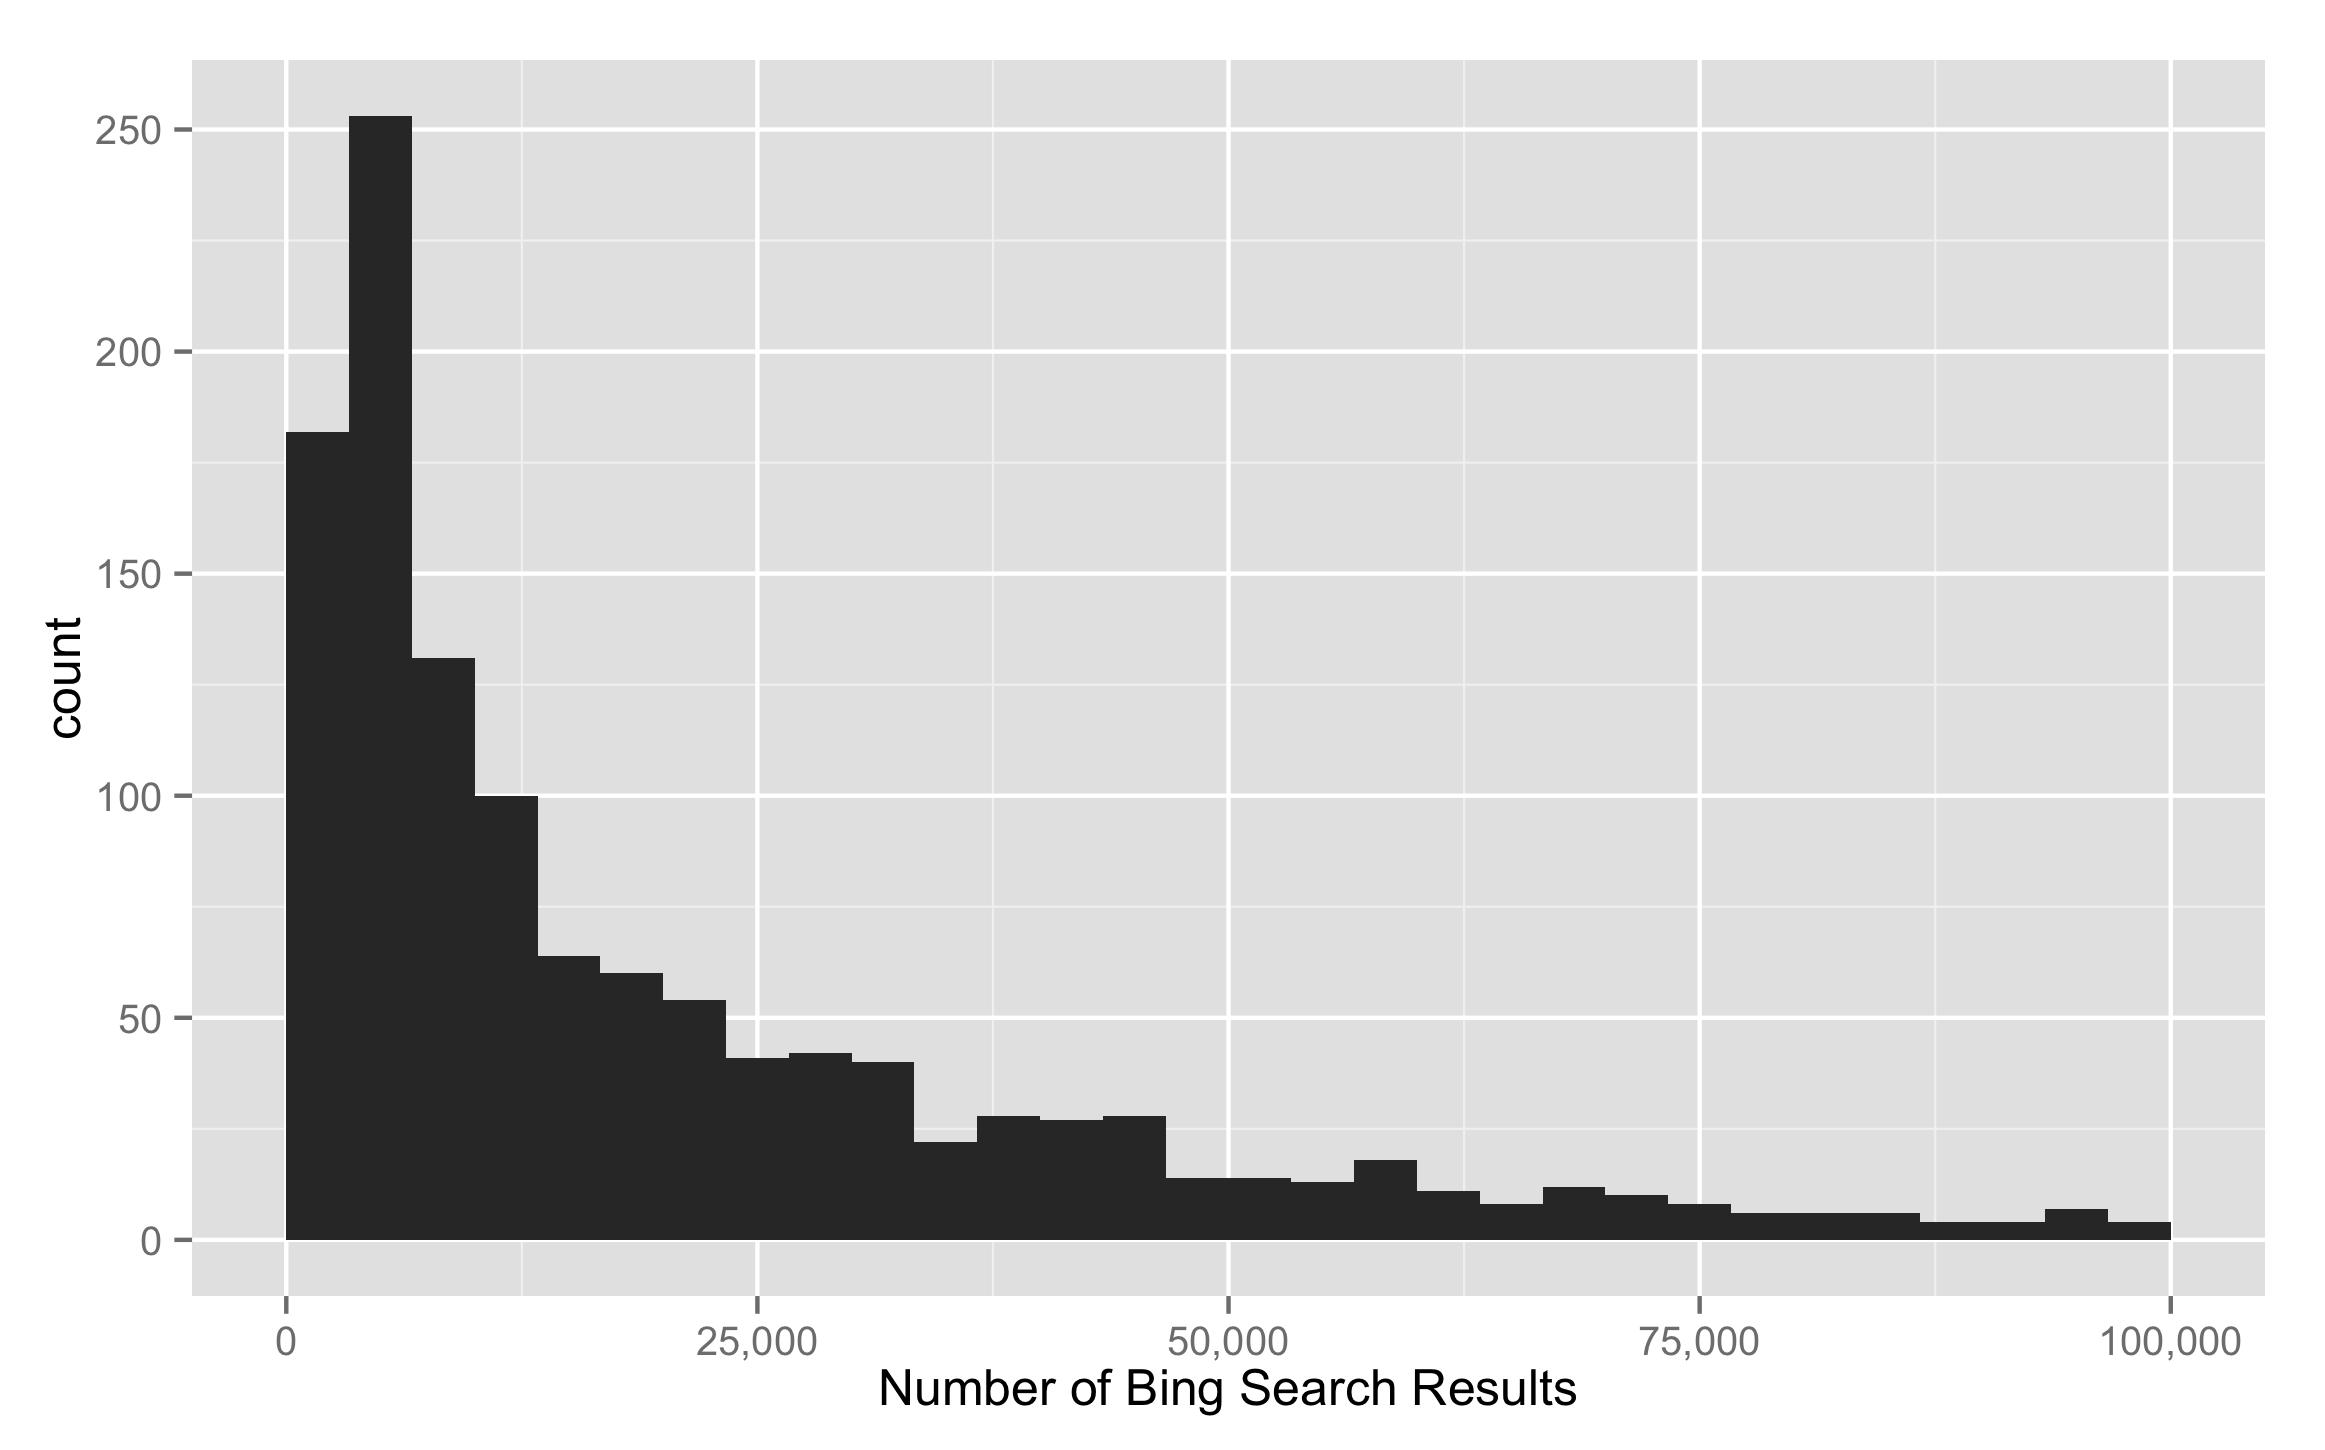
\includegraphics[width=\linewidth]{author_popularity_histogram.png}
\caption{Histogram of Bing Search Results}
\label{fig:ap_hist}
\end{figure}

\begin{figure}[ht]\centering
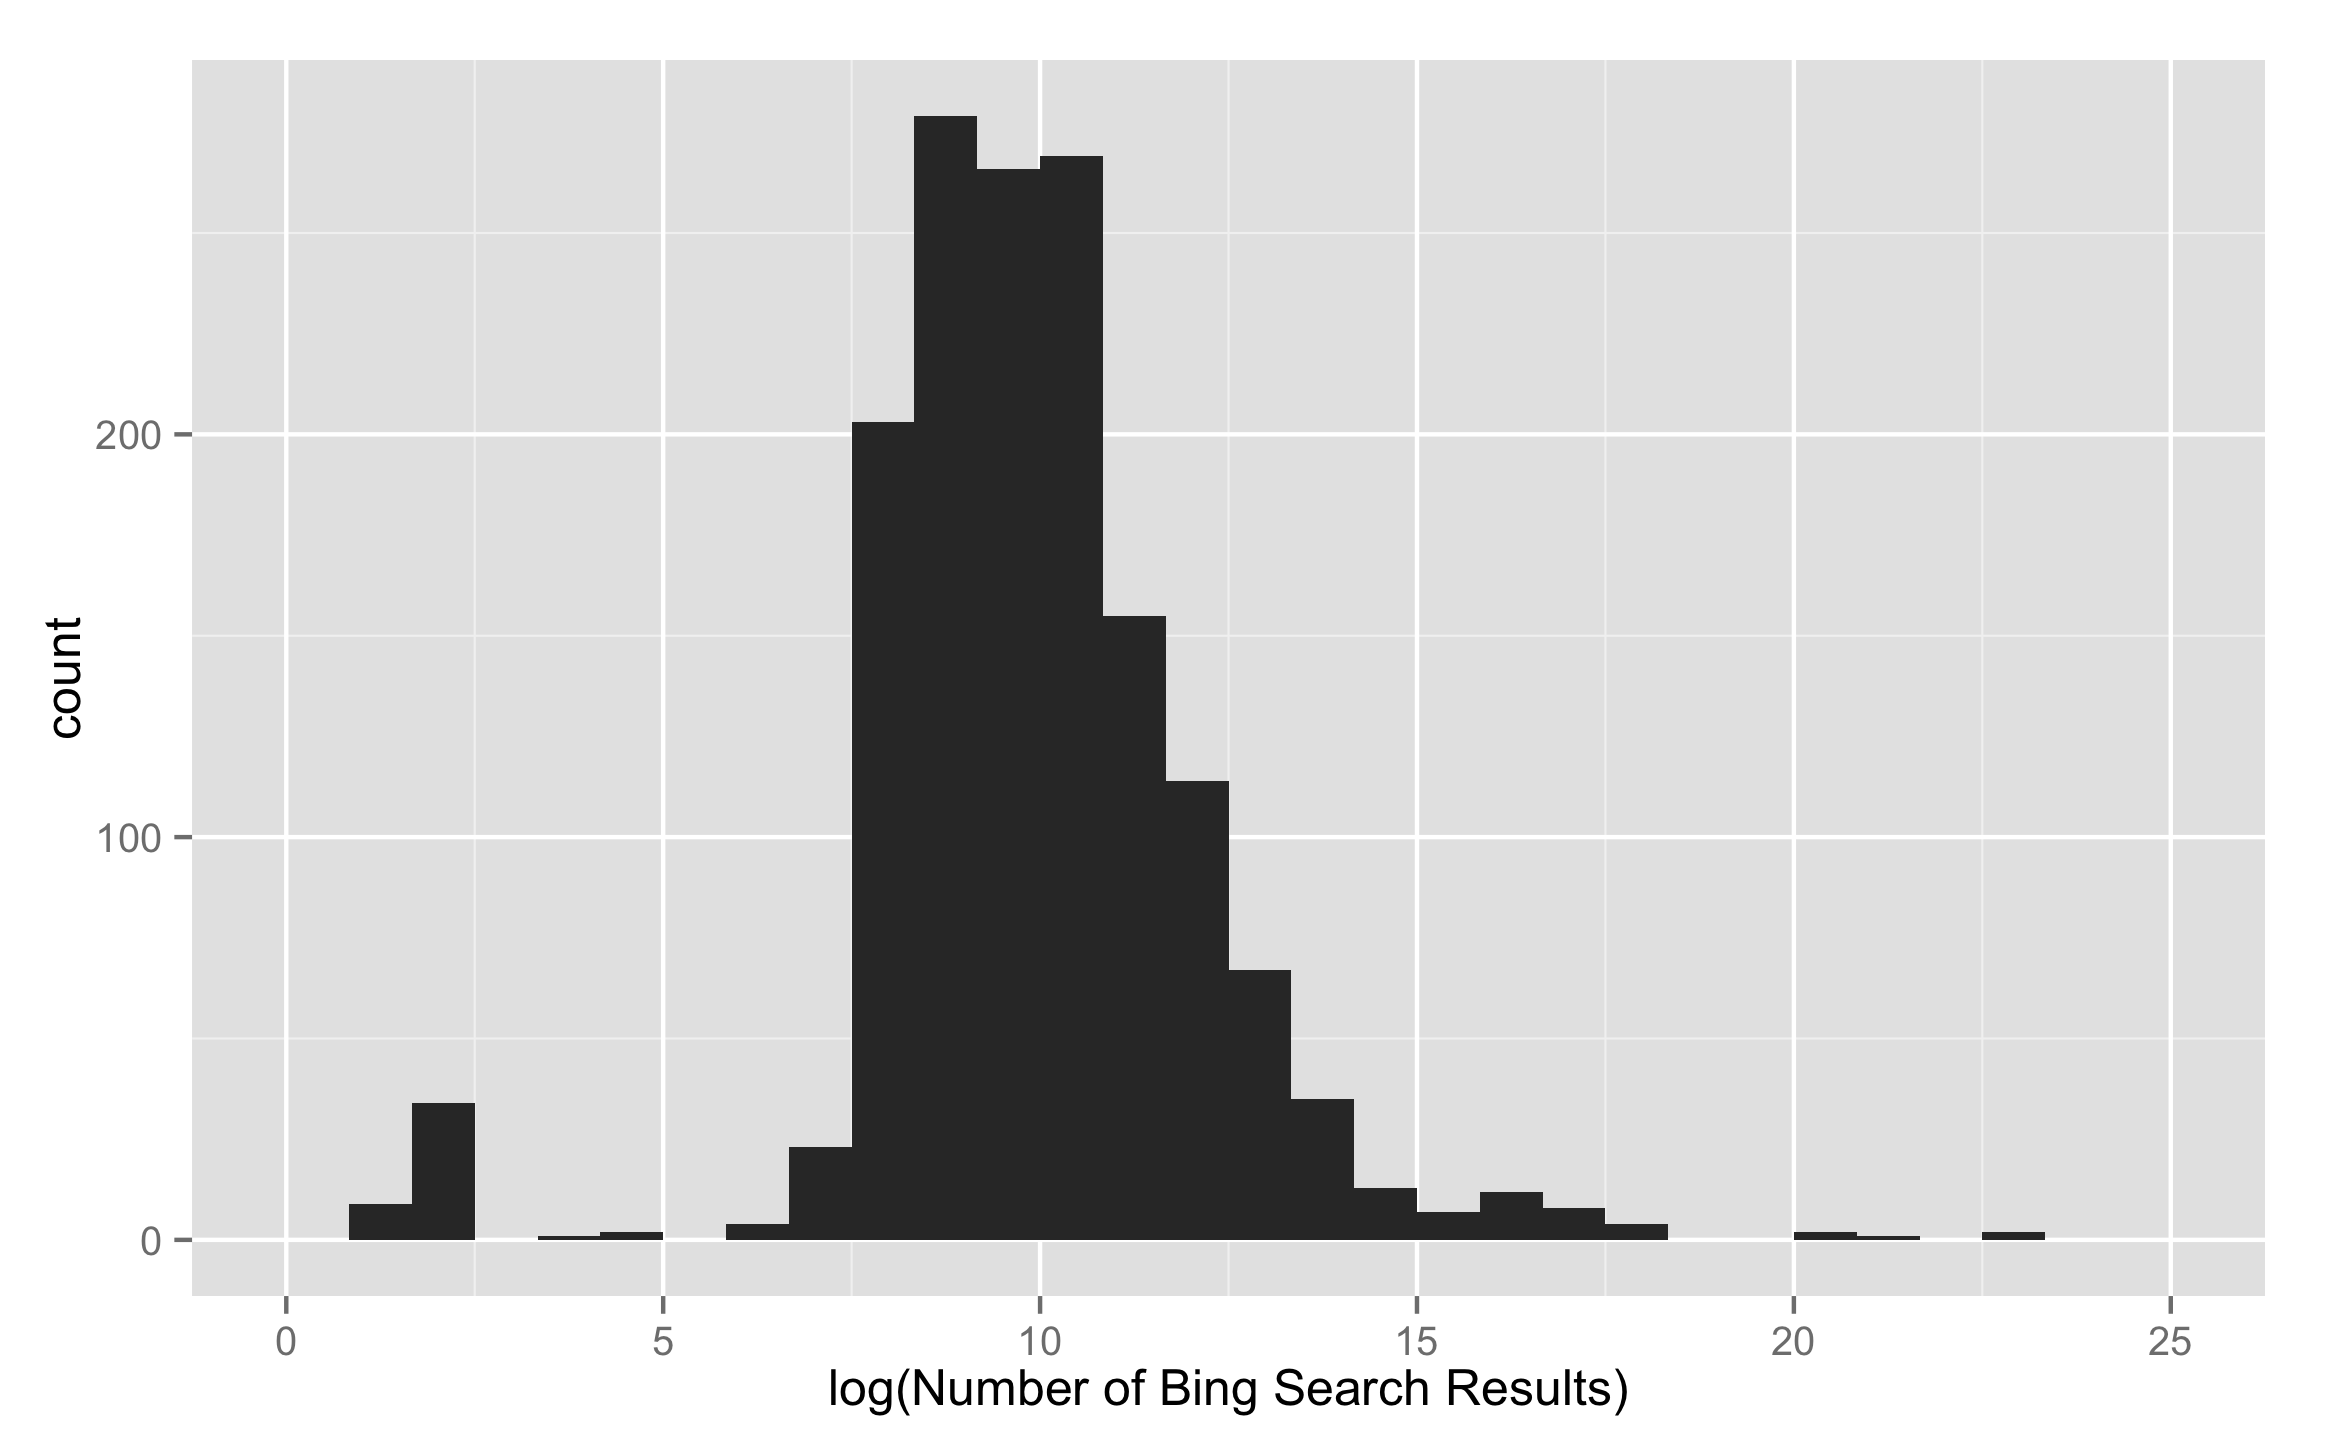
\includegraphics[width=\linewidth]{author_popularity_log_histogram.png}
\caption{Histogram of log(Bing Search Results)}
\label{fig:apl_hist}
\end{figure}
	
\begin{figure}[ht]\centering
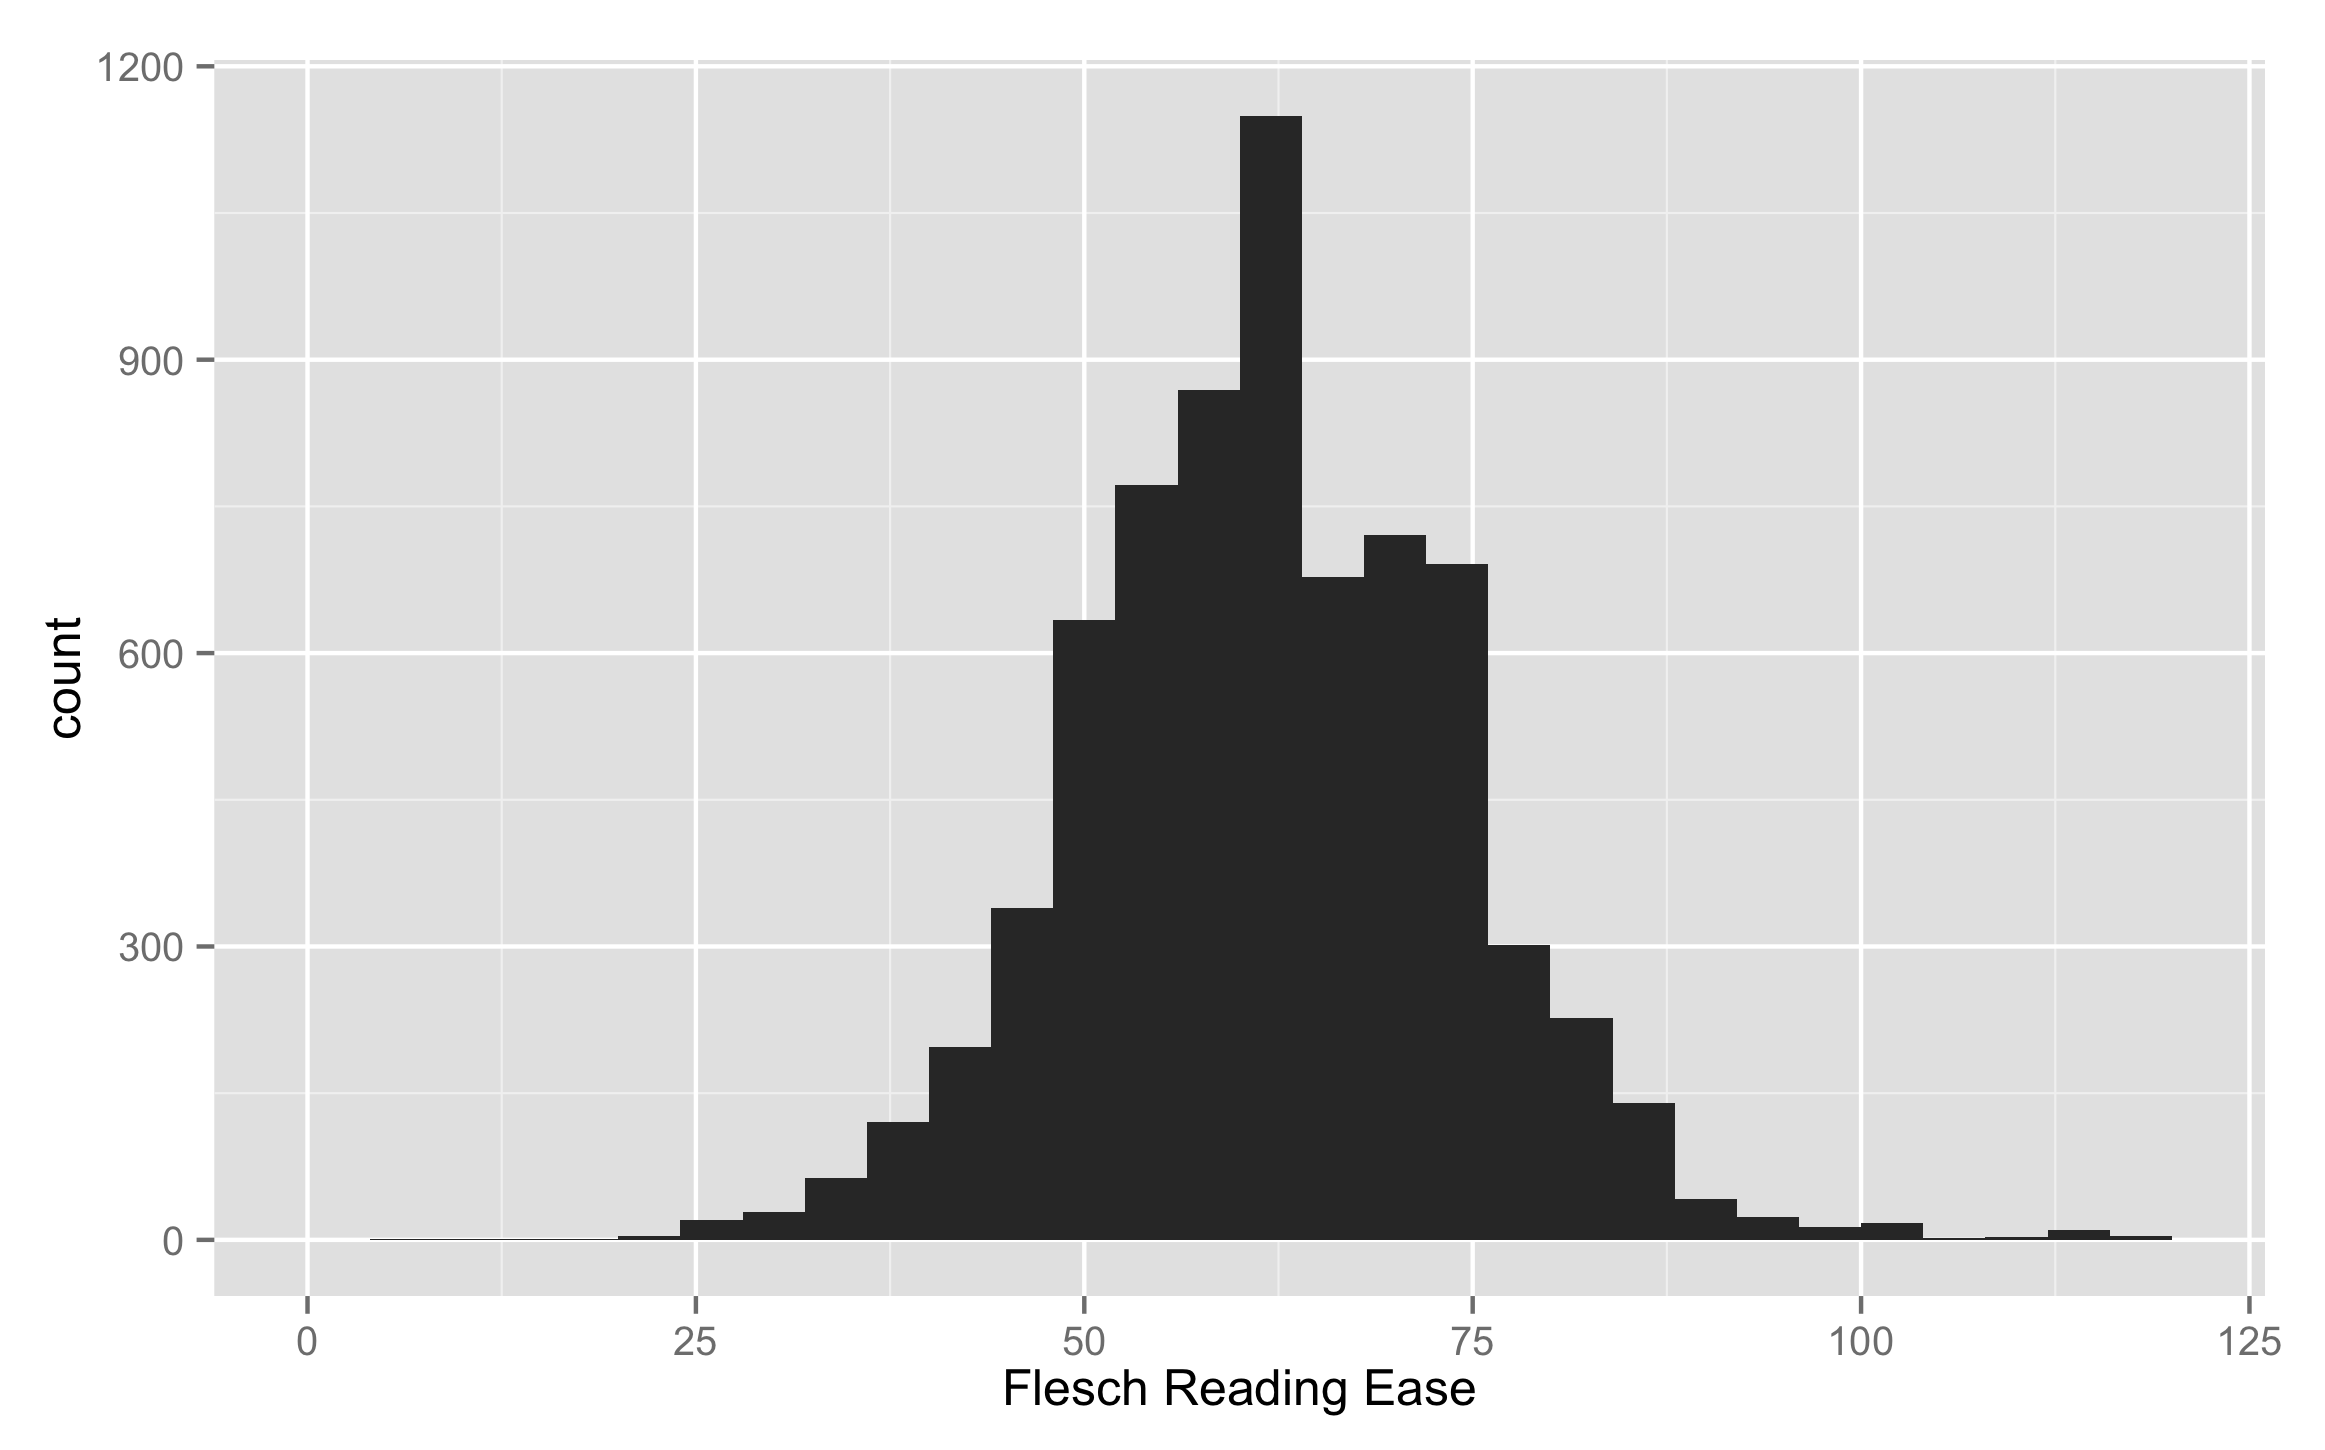
\includegraphics[width=\linewidth]{flesch_data_histogram.png}
\caption{Histogram of Flesch Reading Ease}
\label{fig:fre_hist}
\end{figure}	
	
\end{description}

We also include features that attempt to capture the article sentiment and the article text perplexity. Since the construction of these features was more involved and involved validation of our algorithms, we discuss these two features in separate subsections.

\subsection{Article Sentiment}

In order to measure article sentiment, we use a Naives Bayes text classification algorithm, as described in Rennie et al (2003) \cite{rennie2003tackling}. We assume that each article in our corpus can belong to one of three classes - `negative' sentiment, `neutral' sentiment, and `positive' sentiment, which we will denote as $C_k$. The Naive Bayes model assumes that the likelihood of observing a given article $\mathbf{x} = (x_1, ..., 1_n)$, where $x_i$ is the number of times that word $i$ appears, is 

\begin{equation}
p(\mathbf{x}|C_k) = \frac{\left ( \sum_i x_i \right )!}{\prod_i x_i !} \prod_i p_{ki}^{x_i},
\end{equation} 

\noindent where $p_{ki}$ is the probability of a document of class $K$ including word $i$. Given that we transform this problem into log space, we can compute $\log(p(\mathbf{x}|C_k))$ as 

\begin{equation}
\log(p(\mathbf{x}|C_k)) = \log ( p(C_k)) + \sum_{i=1}^n x_i \cdot \log(p_{ki}).
\end{equation}

We coded up a basic implementation of the Naive Bayes algorithm, drawing heavy inspiration from Greg Lamp's 2014 python tutorial on Naive Bayes \cite{NaiveBayes}. In order to get the probabilities $p(C_k)$ and $p_{ki}$, we developed a training set of NY times data by providing 200 articles to workers on Amazon Mechanical Turk. Each turker was asked to score the sentiment toward the subject of the article in question on a scale from -2 to +2, with -2 being extremely negative and +2 being extremely positive. We recorded 5 scores for every article, and calculated the average sentiment reported by the Turkers. We classified any article having an average score greater than 0.5 as `positive'. Any article with an average sentiment less than -0.5 was `negative.' Any other articles were classified as `neutral.' Ultimately, our labels were 66\% neutral, 14.5\% negative, and 19.5\% positive. This is unsurprising, as a newspaper such as the New York Times likely strives for neutrality when reporting on most topics.

We wanted to determine how our Naive Bayes implementation did compared to an off-the-shelf implementation of the same algorithm. In order to do so, we trained NLTK's multinomial Naive Bayes classifier on the same training data, and then evaluated the sentiment of 1,000 articles. A comparison of the two implementations is found below, where the columns indicate the prediction by the NLTK Naive Bayes implementation and the rows indicate the prediction by our implementation:

\vspace{10 mm}

\begin{tabular}{l | r r r}
\toprule
  & negative & neutral & positive\\
\midrule
negative & 0 & 54 & 0\\
neutral & 2 & 894 & 0\\
positive & 0 & 50 & 0\\
\bottomrule
\end{tabular}

\vspace{10 mm}

Overall, we find 89.4\% agreement between the two algorithms. However, alarmingly, the NLTK implementation seems to predict neutral an overwhelming percentage of the time (99.8\% of the time). This warrants further investigation, and may be due to small differences in implementation, or peculiarities in the sample of 1,000 articles we chose to compare the two algorithms across. In any case, our algorithm seems to be performing in the same neighborhood as the NLTK implementation (if not better), so we feel relatively comfortable moving forward using our sentiment labels.

\subsection{Article Perplexity}
In order to determine the perplexity score, we first need to build some language model that gives us the probabilities of each word. While perplexity typically is a measure of how well a probability distribution can predict a sample, in our context, we interpret perplexity essentially as a measure of article “uniqueness”. The argument here is that if our language model can’t predict the language used in article very well, then the language used in the article is atypical relative to the corpus used to build the language model. Hence, given some language model, an article's perplexity is given by:
\begin{equation}
	2^{-n\cdot\sum_{i=1}^n \log p(w_i)}
\end{equation}
where $n$ is the length of the article, and $p(w_i)$ is the probability of the $i$-th word in the article. We think that perplexity might have some predictive power since people generally have a preference for novelty. If many news articles about the same story are all using highly similar language, an article that covers the story using atypical language is likely unique in some way or another which may drive people to read it more or less.

As for out paper, we consider a couple of choices for our language model. First, we build a simple bi-gram language to establish a baseline. We also build more sophisticated word vector based n-gram neural network language models.

We split our articles into training (~70\%), validation (~15\%), and test sets (~15\%). We build our language model corpus only from the text of the articles in the training dataset. In order to keep the size of our vocabulary relatively manageable, we ignore any case sensitivities (so ``Cat" is the same as ``cat"). Furthermore, we only include a word if it appears at least 5 times. Words that don't make this cutoff are mapped to a generic ``rare word" indicator. Lastly, we also map any numbers (that is actual numbers with digits, not number written with words) to a generic ``number" indicator. This leaves us with a vocabulary size $|V|$ of 29359. To estimate a bigram model, we simply need to compute the counts in our training corpus. Specifically, the probability of some word $w_i$ conditional on its preceding word $w_{i-1}$ is given by:
\begin{equation}
p(w_i|w_{i-1}) = \frac{\textnormal{count}(w_{i-1},w_i)}{\textnormal{count}}
\end{equation}
However, its reasonable to expect that there might be bigrams in the development or test corpora that aren't observed in the training corpus. If this is the case, then any article with an unobserved bigram would be assigned a predicted likelihood of 0. Needless to say, this is very bad. In order to avoid this issue, we apply a technique called add-$\alpha$ smoothing. Essentially what add-$\alpha$ smoothing does is it adds (possibly fractional) counts to every single possible bigram. After smoothing, no bigram, given a fixed vocabulary $V$, will ever have 0 probability. This changes our our estimated word probabilities to:
\begin{equation}
p(w_i|w_{i-1}) = \frac{\textnormal{count}(w_{i-1},w_i) + \alpha}{\textnormal{count} + \alpha |V|}
\end{equation}
This smoothing actually has quite a nice Bayesian interpretation as well. In the bigram case, we can say that words follow a multinomial distribution conditional on its preceding word. The smoothed language model 

Essentially, is we're applying a symmetric dirichlet prior with parameter $\alpha$ to each of these multinomial distributions. 

We use our validation set to determine the optimal value of of $\alpha$ by seeing what value of $\alpha$ minimizes the negative average log-likelihood per word (NALL) of our validation corpus:
\begin{figure}[ht]\centering
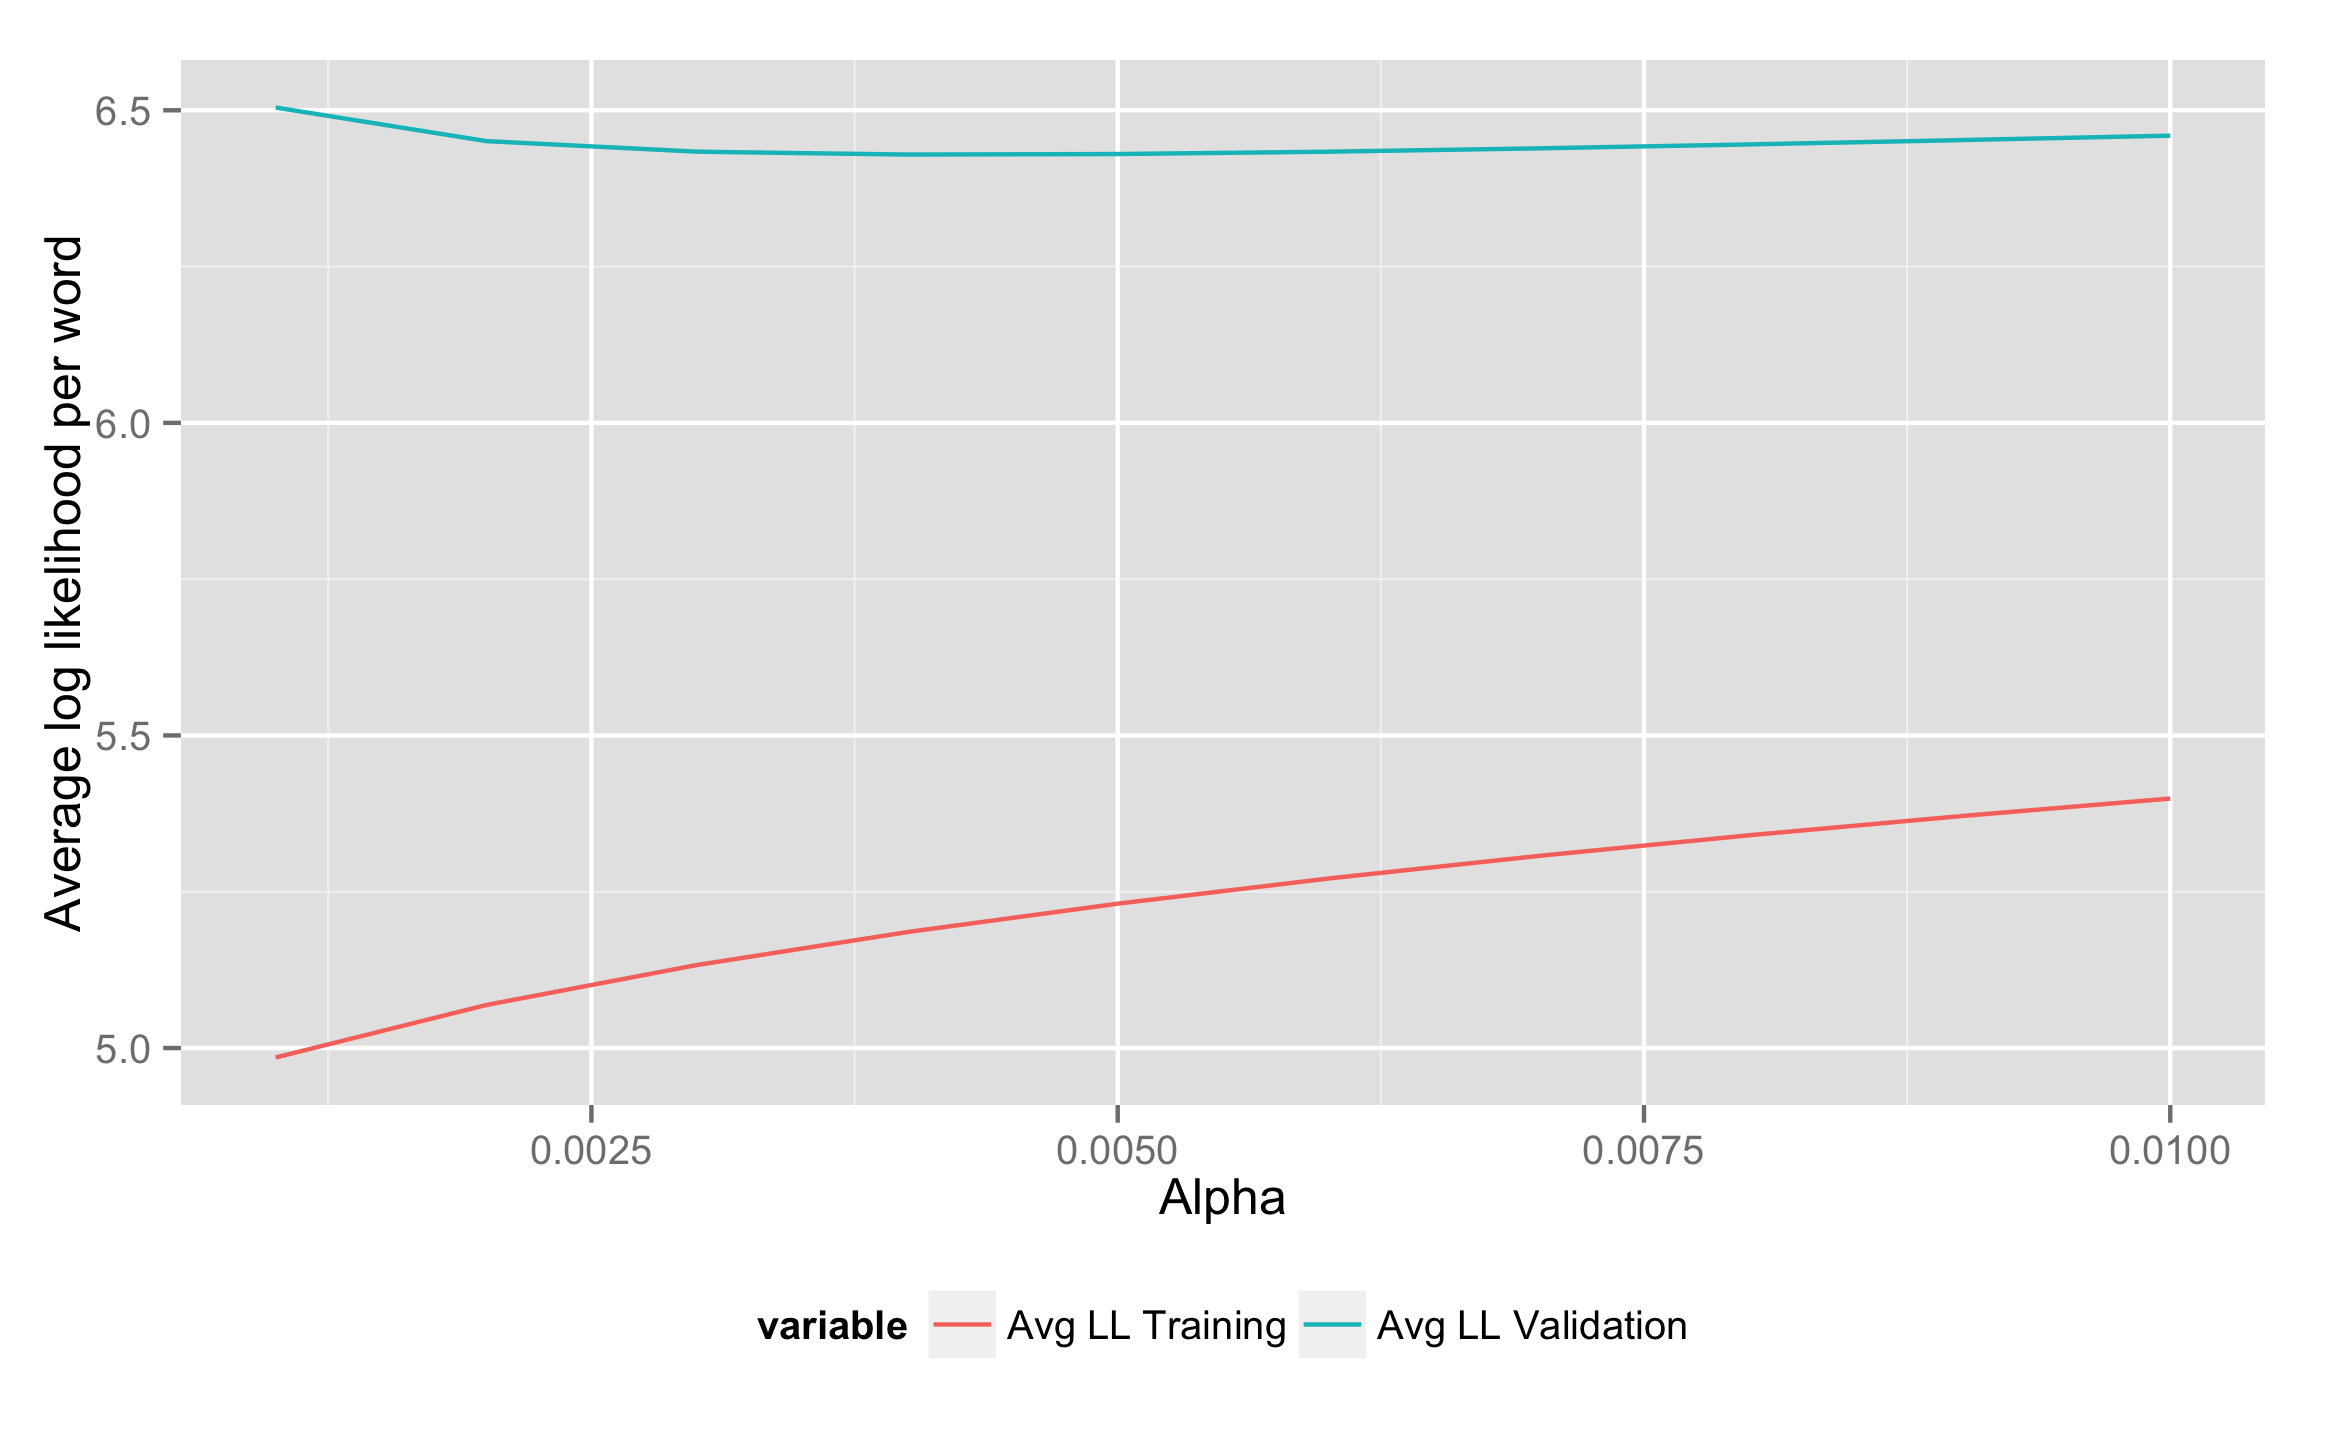
\includegraphics[width=\linewidth]{bigram_add_a.png}
\caption{Negative Average Log-Likelihood per Word as a Function of $\alpha$}
\label{fig:fre_hist}
\end{figure}
Here we see exactly what we should expect. The NALL on the training corpus is lower than the NALL on the validation corpus. Furthermore, the NALL on our training corpus monotonically increases as we increase $alpha$ while the NALL on the validation corpus initially decreases hits a minimum, and starts to increase. For our language model, the optimal $\alpha$ is 0.004. This produces the following NALLs for our 3 corpora:

\begin{table}[hbt]
\caption{Bigram Language Model with Smoothing Negative Average Log-Likelihood}
\centering
\begin{tabular}{ccc}
\toprule
Training &  Validation & Test\\
\midrule
4.98487 & 6.42916 &  6.41888\\
\bottomrule
\end{tabular}
\end{table}

\begin{figure}
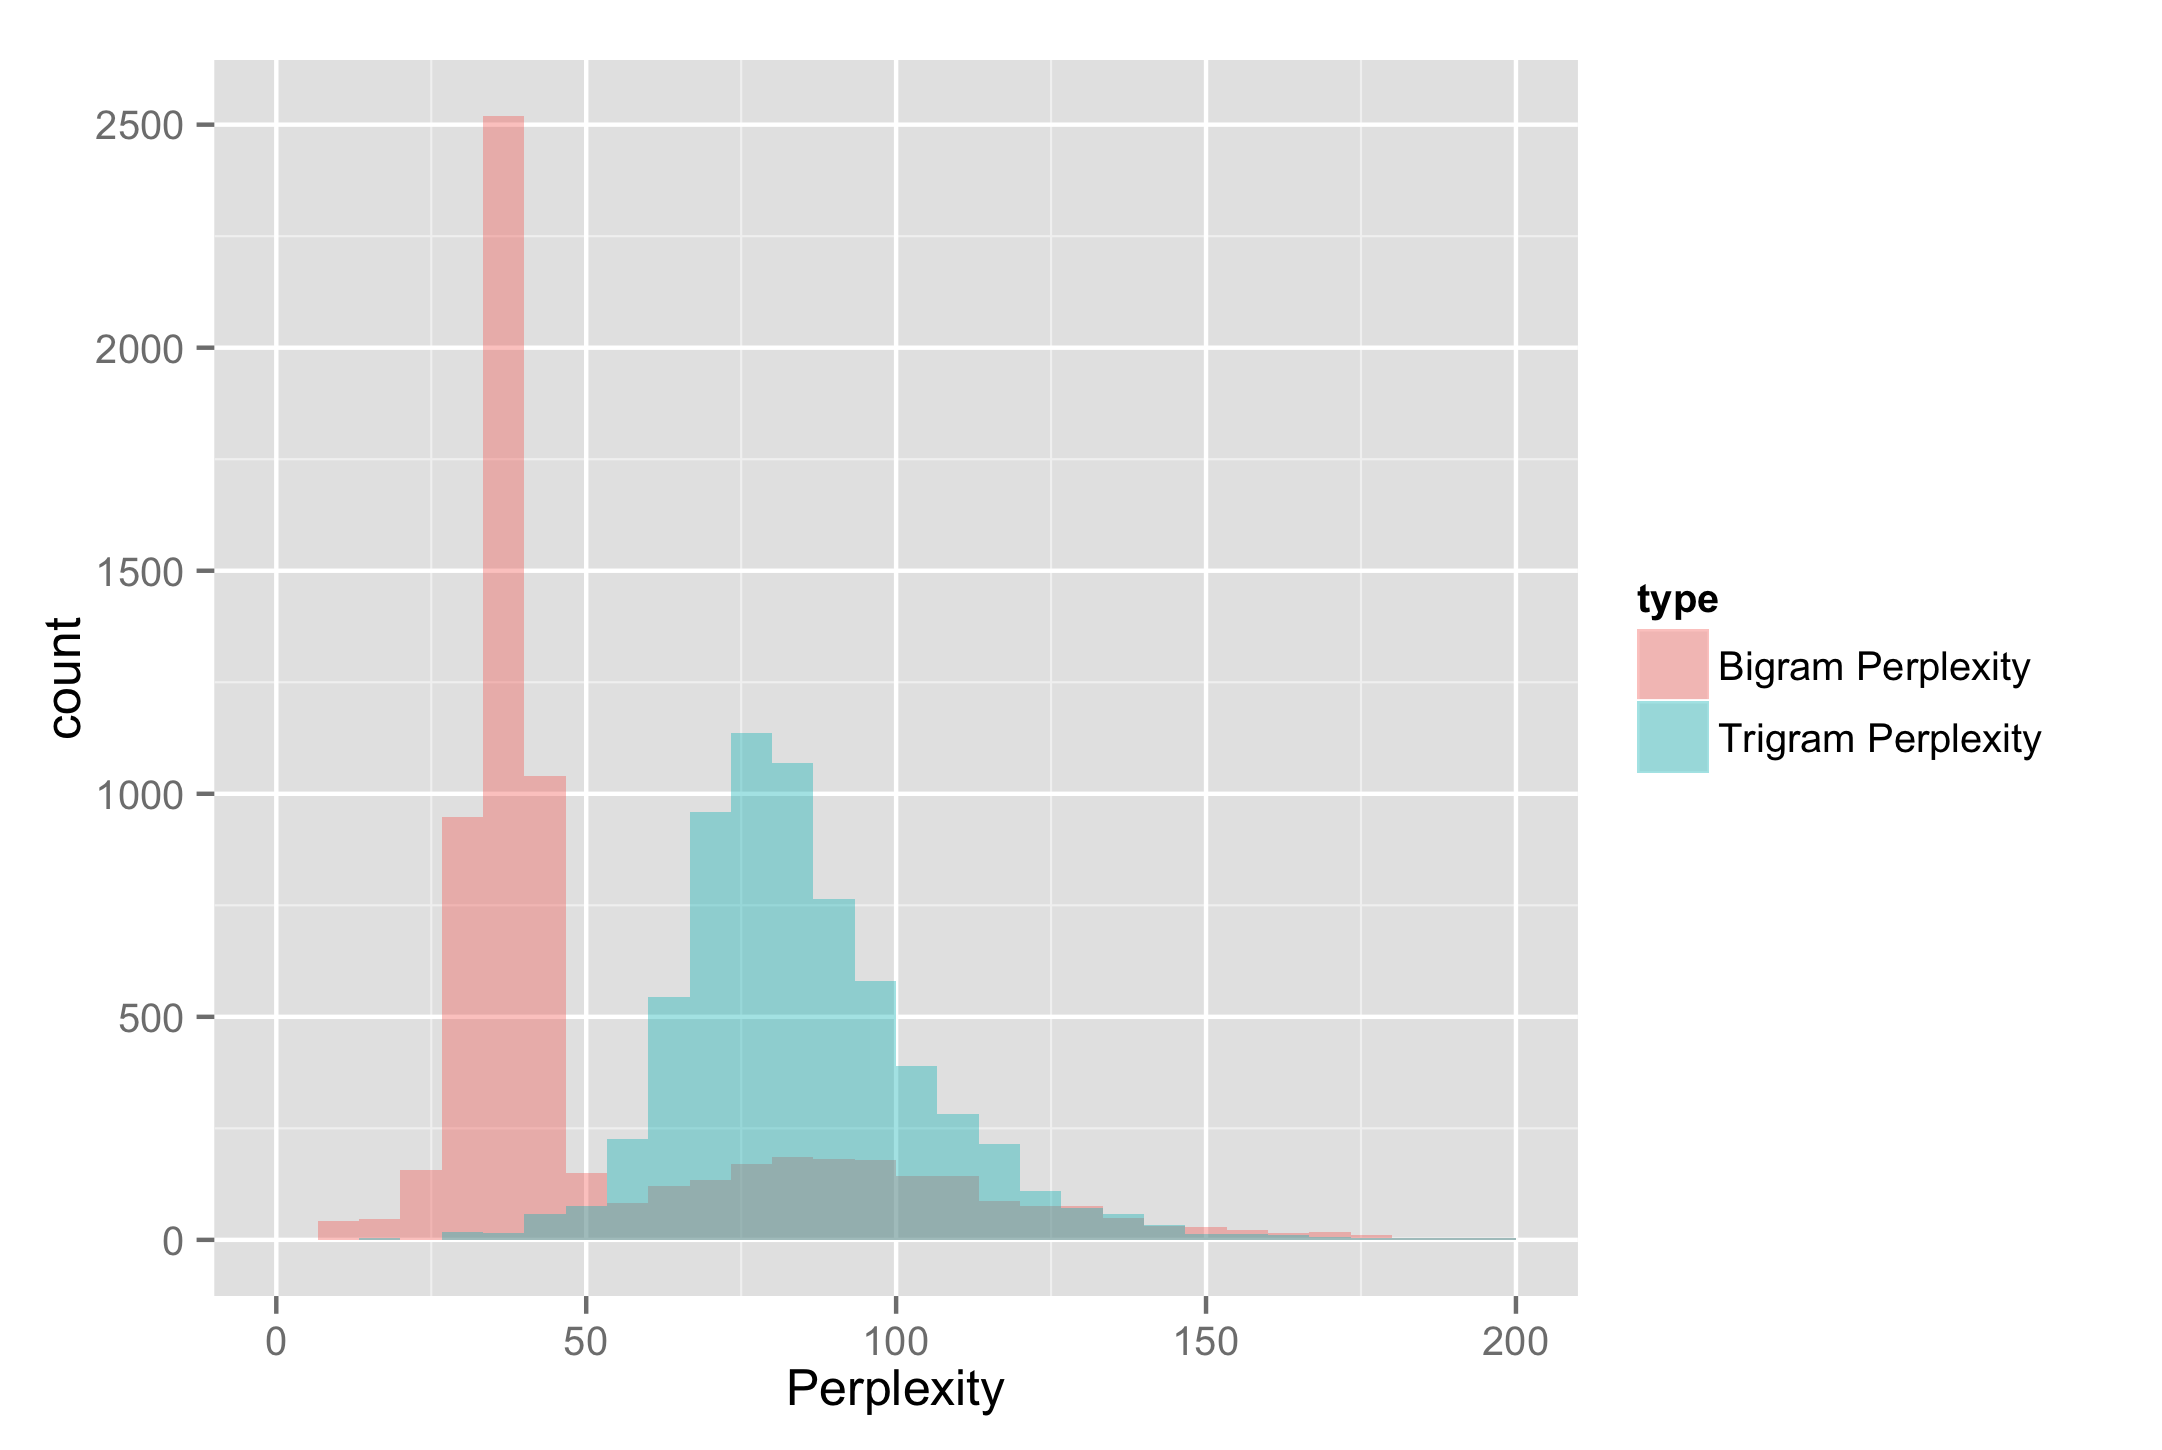
\includegraphics[width=\linewidth]{perplexity.png}
\caption{The distribution of bigram and trigram perplexities}
\label{fig:perp_hist}
\end{figure}

One criticism of standard n-gram language models is that they are rather sensitive to the training data. Suppose that two words generally have fairly interchangeable use cases (meaning that the same or similar words tend to appear before these words), for example, ``coffee" and ``tea". Further suppose that for whatever reason, the phrase ``drink coffee" is predominantly featured in the training data but ``drink tea" is not. Then a standard bigram language model would assign a very low probability to ``drink tea" even if the in the training data contains many instances in which they are fairly interchangeable (``buy coffee/tea", ``brew coffee/tea", etc.).

Hence, we build word vector n-gram neural network models to see if we can achieve better performance. By using dense word vectors rather than one-hot encodings to represent words, we're able to more accurately represent the ``similarity" of words. For example, ``coffee" is more similar to ``tea" that it is to ``car". Rather astonishingly, these word vector values can be trained through back propagation just like the weights in a neural network just as long as they're randomly initiated! 

 In particular, we train both a bigram neural network language model and a trigram neural network language model. In both cases, we use word vectors of length 10 (so for the bigram NN, our input layer is size 10 and for the trigram NN, the input layer is size 20) that map to a single hidden layer with 10 hidden units with a tanh activation function. The hidden layer is then connected to the output layer which is the size of our vocabulary with a softmax activation function. Given that we want to also train our word vectors, we use stochastic adaptive gradient descent. We purposefully keep our network relatively small since our data set is rather large and training even this small neural network takes considerable time. 
 
 Unfortunately, our neural networks are still in the process of training. Due to various complications, we were not able to train our model for as long as we would've liked. Couple this with the fact that our training corpus contains over 3,000,000 observations and each complete pass through it takes approximately 4.5 hours, means that as of writing this paper, we've only completed 4 full passes. Unfortunately, as a result of an oversight in the code, we forgot to store the NALL of training data as we complete each full loop. However, we are highly confident our neural network is working as intended since we see we that the NALL decreases every pass on the validation corpus:
 
 %% GRAPH AND TABLE HERE
 
We fully expect the validation corpus NALL to eventually start increasing once the neural network begins to overfit the training corpus, however we simply haven't reached that point yet. 
 
Despite the fact that our training isn't finished, both our neural network-based language models are already performing better than a standard bi-gram model with smoothing. We build 2 sets of article perplexity scores. One set is derived from the smoothed bigram model to serve as a base comparison. Our other set is derived from the most recently completed pass of our trigram NN language model. We report the following article perplexity scores distribution:

%

%% PUT PERPLEXITY DISTRIBUTIONS HERE

%

Its important to note however, that we don't necessarily care exactly how good our language model. Since we only use the language model as an intermediate step to construct a feature for a regression task. It could very well be the case features generated by a worse language model can work just as well as well in the regression task as features generated by a better language model if the relative variation of articles is maintained. To test whether a better language model can give us more predictive power, we compute two sets of perplexity scores, one based on the smoothed bigram language model and one based on the current best trigram neural network language model. 


\section{Predictive Regression Model}

Once we have constructed our full set of features, we aim to predict log(article pageviews), $\mathbf{y}$, using our full set of variables, which we include in our design matrix, $\mathbf{X}$. We estimate the feature weights using the closed form solution for both OLS and ridge regression:
\begin{equation}
\beta = (\mathbf{X}^T\mathbf{X} + \lambda \mathbf{I})^{-1}\mathbf{X}^T\mathbf{y}
\end{equation}
where $\mathbf{I}$ is the $k \times k$ identity matrix, and $\lambda$ is our regularization parameter. Setting $\lambda = 0$ corresponds to OLS, whereas non-zero values of $\lambda$ correspond to ridge regression. The motivation for performing ridge regression as opposed to OLS is to not overfit on our data. 

In order to choose an appropriate value of $\lambda$, we split our data into a training and validation set. 90\% of the data is allocated to the training set, and 10\% of the data is allocated to the test set. We cross-validate the estimated $\beta$ values on our validation set for each $\lambda$, and choose the value of $\lambda$ that produces the lowest MSE on the validation data.

The table below displays the 20 feature weights with the largest magnitudes given our model. A bar chart showing the magnitude of all of the weights (excluding the intercept weight) can be found in Figures \ref{fig:lin_reg_weights1} and \ref{fig:lin_reg_weights2}.

\begin{table}[hbt]
\caption{20 Most Significant Weights}
\centering
\begin{tabular}{lr}
\toprule
Feature  &  Weight\\
\midrule
intercept & 8.964\\
log(Word Count) & 0.741\\
Desk: Foreign & 0.550\\
Desk: Travel & -0.465\\
Section: World & -0.402\\
Section: Opinion & 0.283\\
Type: BlogPost & -0.282\\
Type of Material: Schedule & -0.267\\
Desk: None & -0.262\\
Section: Movies & -0.239\\
Time of Day: 12-17 & 0.232\\
Type of Material: Review & -0.218\\
Desk: National & 0.211\\
Section: Health & 0.210\\
Section: Books & 0.201\\
Type of Material: Letter & -0.200\\
Type of Material: News & 0.187\\
Section: Sports & -0.175\\
Type of Material: Op-Ed & 0.170\\
Desk: BookReview & -0.154\\
\bottomrule
\end{tabular}
\end{table}

\begin{figure*}[ht]\centering
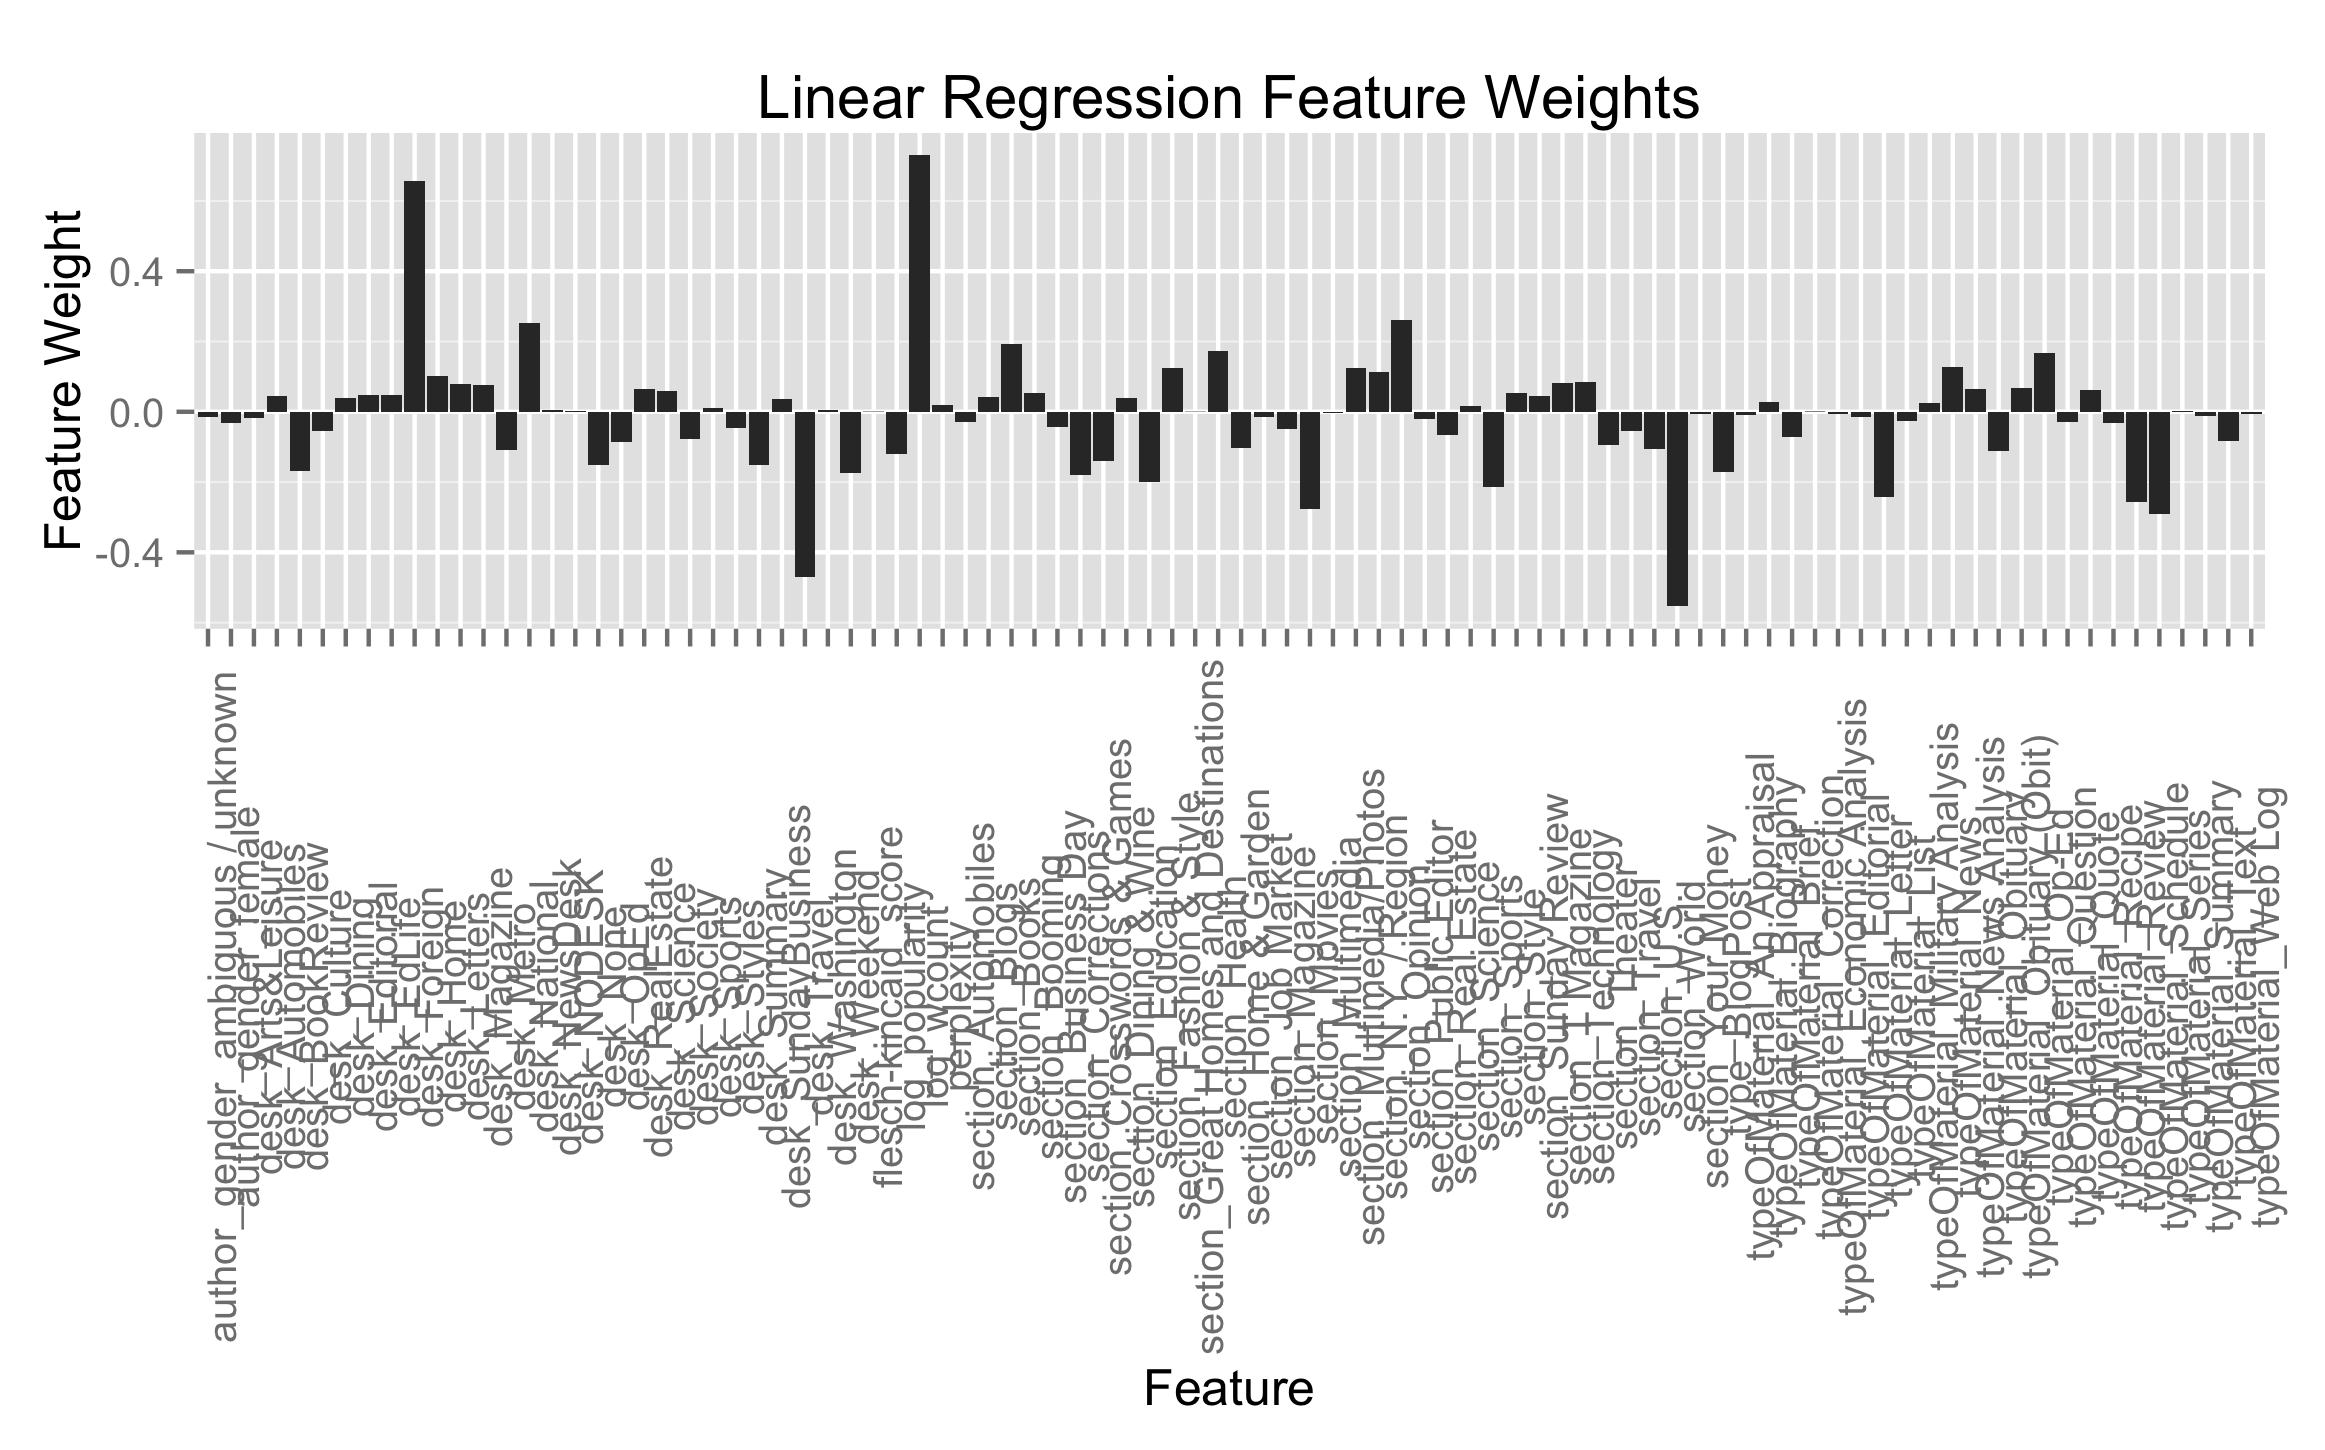
\includegraphics[width=\linewidth]{feature_weights.png}
\caption{Linear Regression Feature Weights (excluding intercept term)}
\label{fig:lin_reg_weights1}
\end{figure*}

\begin{figure*}[ht]\centering
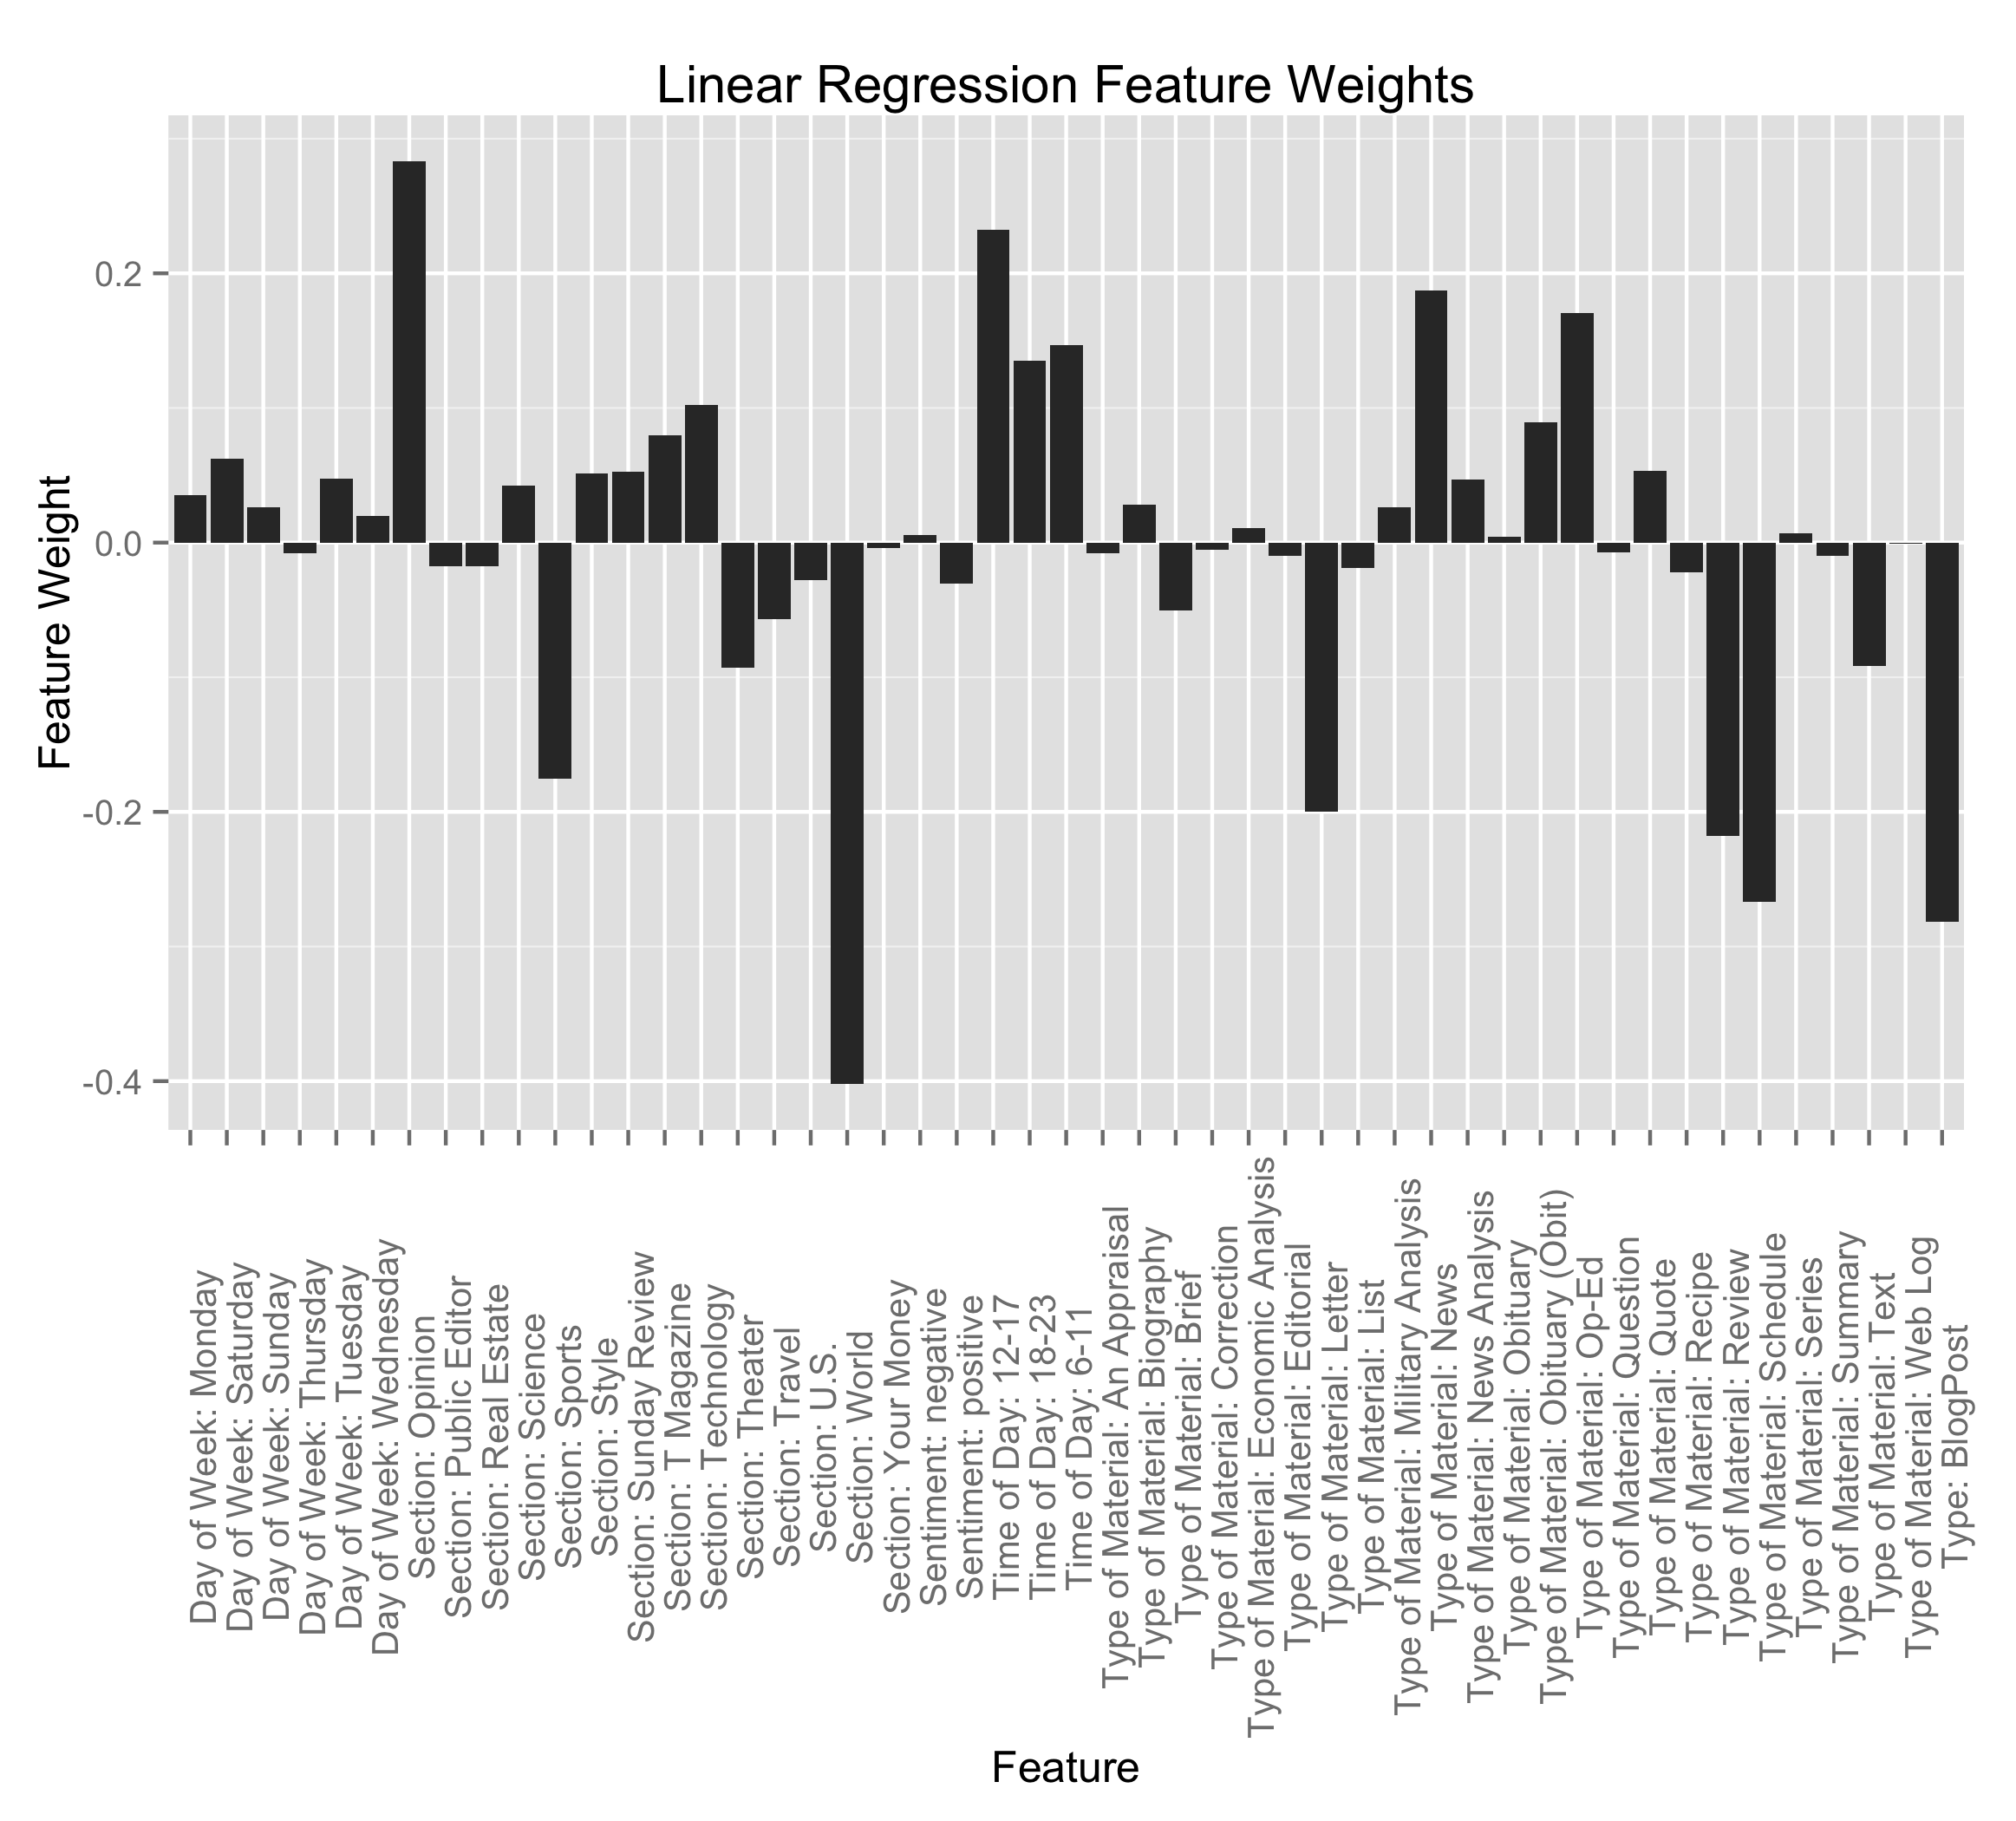
\includegraphics[width=\linewidth]{feature_weights_contd.png}
\caption{Linear Regression Feature Weights (excluding intercept term)}
\label{fig:lin_reg_weights2}
\end{figure*}

Figure \ref{fig:mse_plot} shows the training and holdout MSE for various values of Lambda. There are a few things in this plot worth discussing. First, note that the holdout MSE is consistently lower than the training data MSE. Given the (relatively) small size of our dataset (6,687 observations), this is likely due to the sampling we used to separate our data into training and validation data. However, this shouldn't effect the validity of our cross validation.

Another thing worth noting is that even on the training dataset, the MSE goes down once we choose a non-zero value of $\lambda$. At first, this was surprising to our group, as conceptually OLS is often thought of as the linear regression method that minimizes MSE. However, it is important to note that OLS only holds this distinction amongst unbiased estimators. Hoerl and Kennard (1970) \cite{hoerl1970ridge} prove the existence theorem for ridge regression, which proves that there exists a value of $\lambda$ for which $\beta_{ridge}$ produces a lower MSE than $\beta_{OLS}$. 

Another way of framing this finding is through bias-variance tradeoff. Recall that the MSE can be written as a function of the bias and variance:

\begin{equation}
MSE = (\textrm{Bias})^2 + \textrm{Var}.
\end{equation}

\noindent For some values of $\lambda$, ridge regression is able to lower the MSE by decreasing variance, but adding a non-zero bias term. We believe this is what is happening in our data when cycling through different $\lambda$ values.

\begin{figure}[ht]\centering
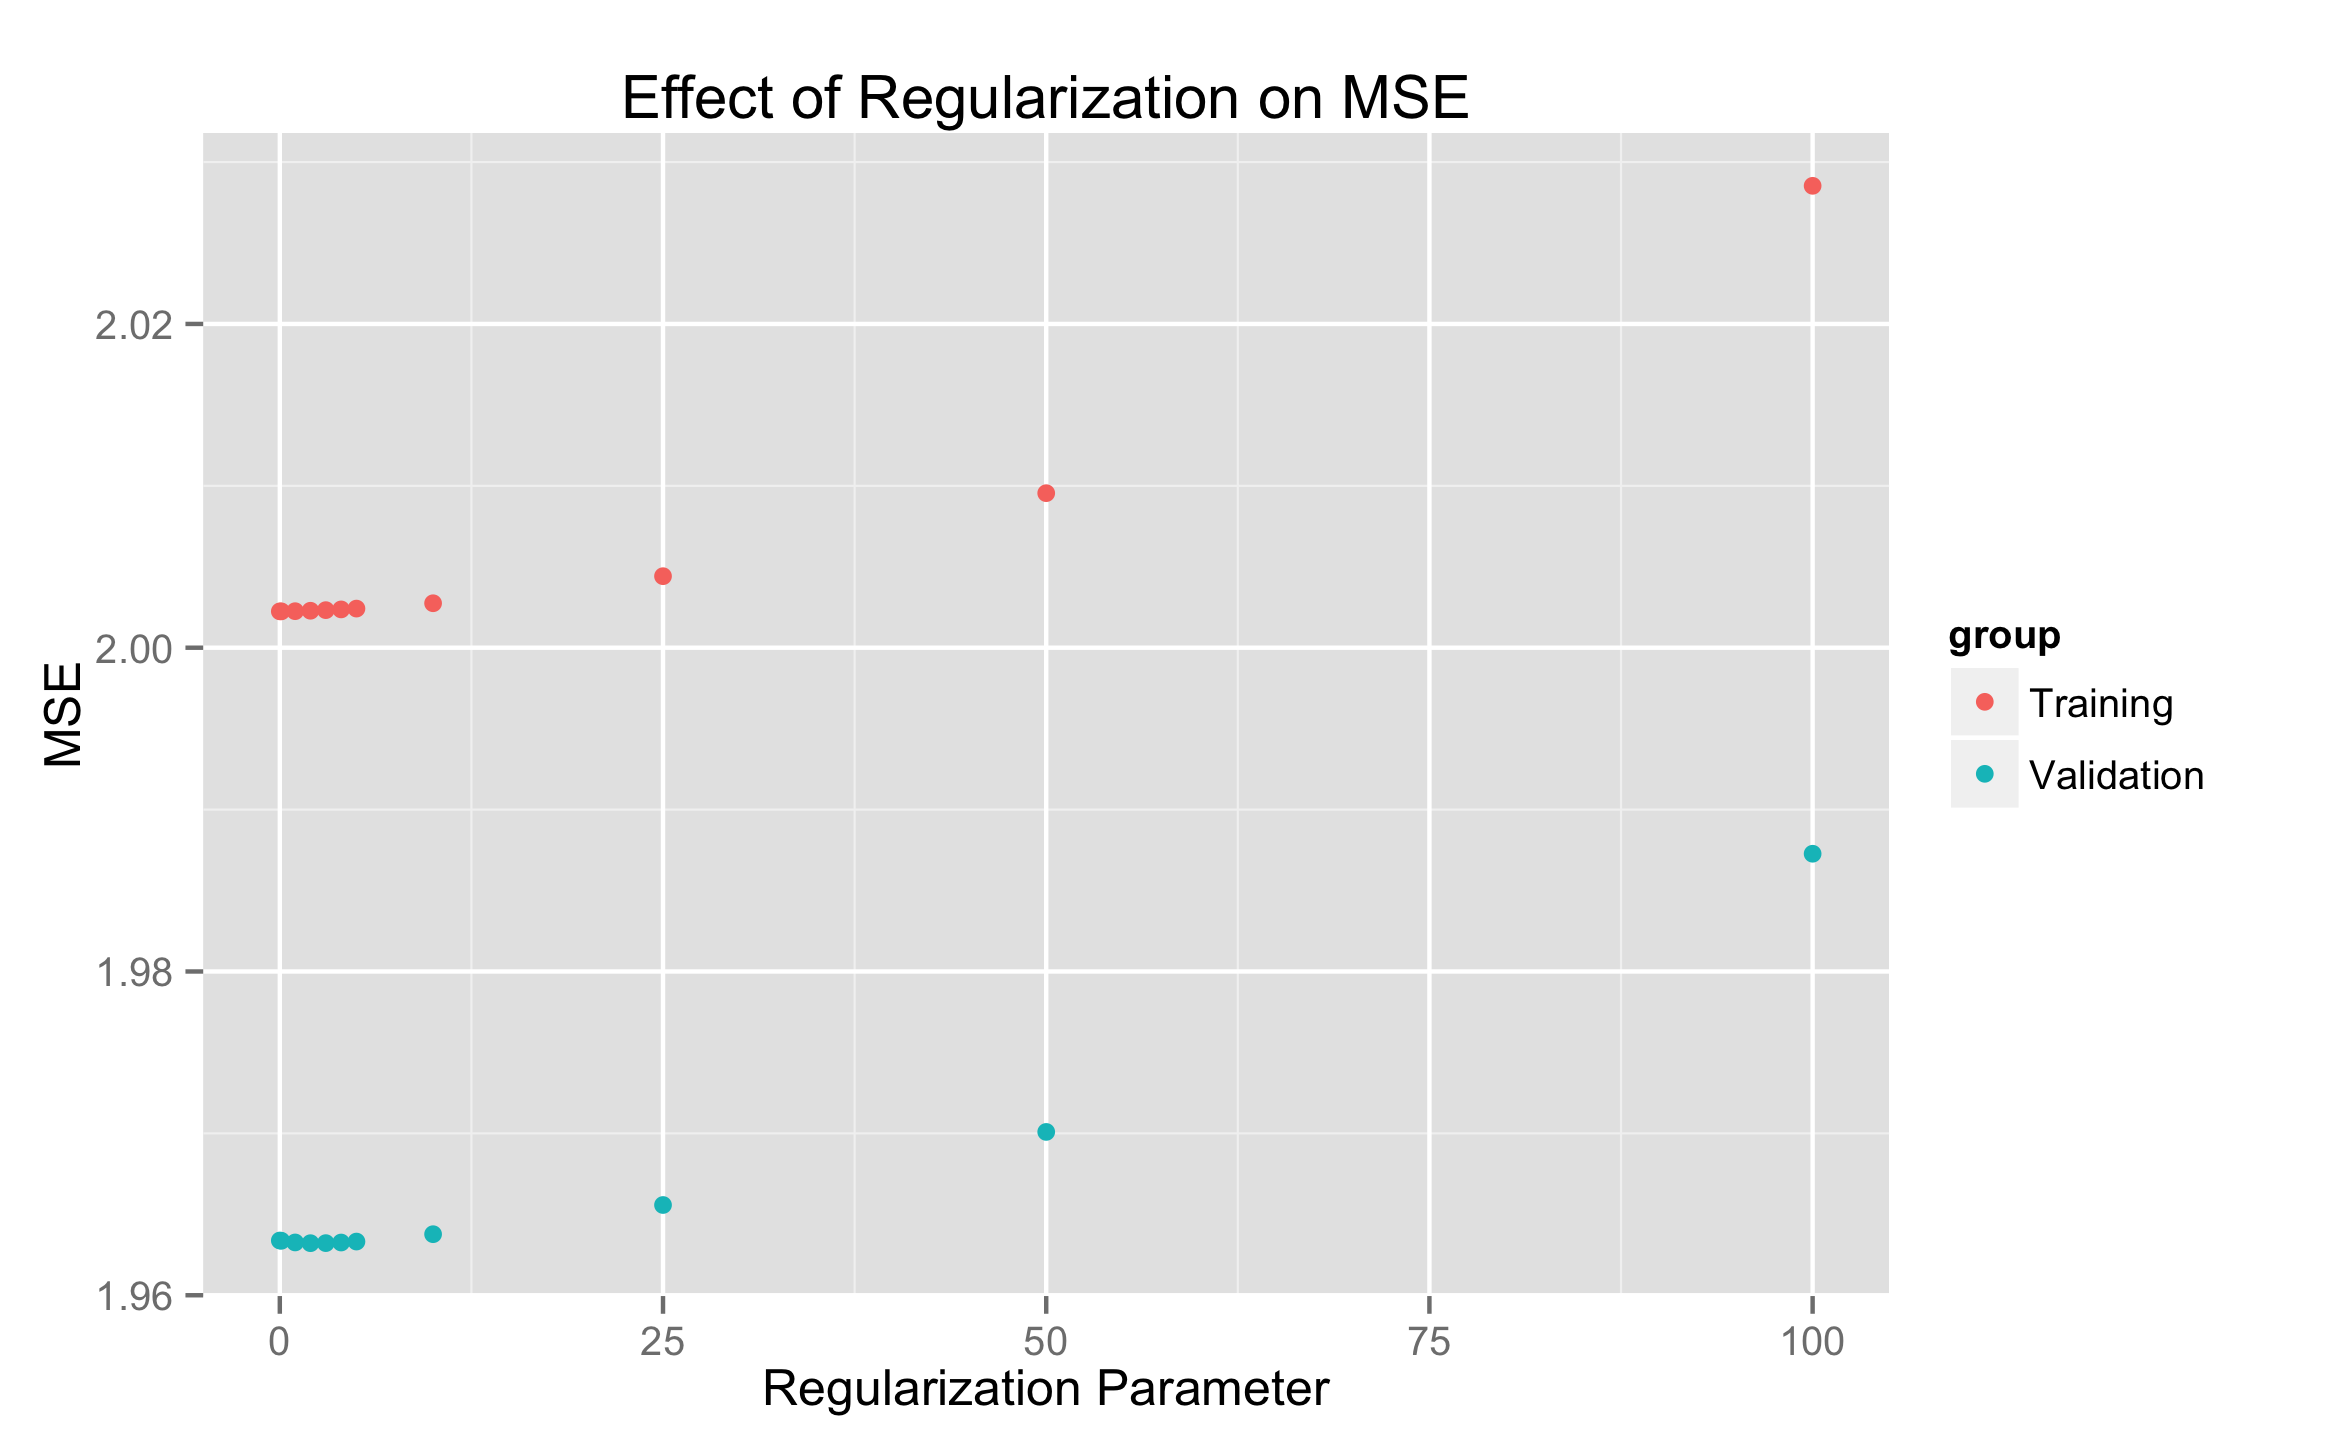
\includegraphics[width=\linewidth]{mse_plot.png}
\caption{The effect of regularization on MSE}
\label{fig:mse_plot}
\end{figure}

\subsection{The Effect of Textual Features}

Given the large amount of work we put into building numerous text-based features (such as the trigram neural network perplexity, the sentiment, and the Flesch reading ease), we may want to evaluate how impactful these various features actually are in our regression. How much incremental reduction in MSE are we getting by including them? We first re-run the exact same regression specification, but instead of using the trigram perplexity calculated from our neural network, we instead use the simple bigram perplexity discussed earlier in this paper. We find that this actually causes the MSE to decrease, from 2.392 to 2.389. This small, but modest change suggests that there is almost no incremental value from the neural network feature.

Now, we might ask if any text features are adding much value. Particularly given that, in general, the magnitude of their weights is dwarfed by the magnitude of the weights of the contextual features when looking at feature weights, we might expect that text features do not add much. When removing perplexity, sentiment, reading ease, and word count features from our regression, we find that the MSE increases, from 2.392 to 2.502. This is result is encouraging, as it suggests that even if text features aren't doing much, they're doing something! Removing them from our model leads to a 4.6\% increase in the MSE.

\begin{table}[hbt]
\caption{Comparison of MSEs for different model specifications}
\centering
\begin{tabular}{cccc}
\toprule
  & NN Trigram & Bigram & No Text\\
\midrule
Best Val. MSE & 2.392 & 2.389 &  2.502 \\
Train. MSE & 2.011 & 2.011 &  2.274 \\
OLS Val. MSE & 2.407 & 2.405 & 2.506 \\ 
\bottomrule
\end{tabular}
\end{table}

\section{Future Work}
Unfortunately due to time constraints as well as various unanticipated difficulties and technical errors, we were unable to implement all of several important features we had initially wanted to include in our regression. Most notably, this paper in its current state lacks some form of topic modeling which we expect to be a strong predictor of content viewership at least in our context. We also think the constructing some features using only the headlines might also provide some improvement, especially considering that an article's headline usually ends up being fairly important in a user's decision to click through or not.

There is also much room for improvement with our existing features as well. For example, the perplexity score feature ended providing very little predictive power might be a result of the underlying language model not being good enough, especially considering that the neural network model still hasn't completed its training. Though we did observe that there was virtually no difference moving from the bigram perplexity scores to the trigram neural network perplexity scores, this again might be because the neural network wasn't given sufficient time to train. We can imagine that if we continued training our neural network for several more cycles, we might start to see visible performance gains. Alternatively, we think its likely the its not the perplexity of an article relative to the entire corpus that matters, but rather perplexity relative to other articles that cover the same event or topic. 

Similarly, there is ample room to improve our sentiment analysis methodologies. The training dataset that we generated using mechanical turk is relatively small (200 articles). Because of this, there are currently many words that may have strong conditional probabilities of appearing given a particular article sentiment that simply do not appear in our training data. With more time (and money!), we might be able to expand the size of our training data and consequently include the accuracy of our model. Furthermore, the model currently skips words it hasn't seen in the training corpus - it might make sense to augment our Naive Bayes implementation to incorporate a method such as Laplace smoothing so as to not simply ignore words we haven't seen in our training data.

Furthermore, the current discrepancies between our implementation of Naive Bayes and NLTK's, while not large in magnitude, are alarming. Given more time in the future, we hope to dig deeper into what is happening. Our current hypothesis is that NLTK's implementation of Naive Bayes does not take into account the number of times a particular word appears in a document. Because of this, more distinct informative words are required to move a given article's prediction away from the neutral class, which has an extremely strong prior.

Another way we could improve our model is to apply a basis expansion to our variables to include polynomial and various interaction terms. In many cases, theres no good justification to why a feature is linearly related to the output feature. Hence, applying a polynomial expansion might uncover an entirely different relationship between our dependent variable and its covariates. We also think that interaction terms might provide some significant predictive power. 

Certainly one thing we definitely plan on doing if we end up trying to turn this project into a publishable paper is to include all of the articles in our dataset. With the much greater sample size and the much more expansive corpus from the additional articles, we might expect to see drastically different optimal weights. 

Since we also have Twitter data that tracks every tweet and retweet involving a NYT article, we would like to extend this project to also include our Twitter data. We can then explore many interesting potential cross effects, such as how does the article content predict the amount of Twitter sharing and alternately, how does content of a Tweet predict viewership.
=======
\section{Division of Labor}

The work for this project was divided as follows. Michael extracted the New York Times contextual data and page view counts and wrote the NYT website scraping script. Dave and Jeremy built out many of the content-driven features and additional contextual features, such as word count, author gender, popularity, and Flesch reading ease. Dave and Jeremy built the implementation and validation of the Naive Bayes classifier, while Michael focused his efforts on the construction and validation of the language model. Dave, along with assistance from Michael, focused on the implementation of OLS and ridge regression, along with validation and discussion of results. Plot generation, table creation, writing, and editing was evenly split between Michael and Extenuating personal circumstances unfortunately prevented Jeremy from contributing to the project as much as originally anticipated.

%------------------------------------------------
\phantomsection
\section*{Acknowledgments} % The \section*{} command stops section numbering

We would like to thank Professor Sinan Aral for his work procuring this dataset, as well as his limitless advice, mentorship, and patience. We'd also like to thank Paramveer Dhillon for his useful comments and his work pre-pre-processing our dataset.

\addcontentsline{toc}{section}{Acknowledgments} % Adds this section to the table of contents

%----------------------------------------------------------------------------------------
%	REFERENCE LIST
%----------------------------------------------------------------------------------------
\phantomsection
\bibliographystyle{unsrt}
\bibliography{Paper}

%----------------------------------------------------------------------------------------

\end{document}